% arara: pdflatex
% arara: pdflatex
% arara: pdflatex

% options:
% thesis=B bachelor's thesis
% thesis=M master's thesis
% czech thesis in Czech language
% slovak thesis in Slovak language
% english thesis in English language
% hidelinks remove colour boxes around hyperlinks

\documentclass[thesis=M,czech]{FITthesis}[2019/12/23]

\usepackage[utf8]{inputenc} % LaTeX source encoded as UTF-8

% \usepackage{amsmath} %advanced maths
% \usepackage{amssymb} %additional math symbols

\usepackage{dirtree} %directory tree visualisation
\usepackage{svg}
\usepackage{float}
\usepackage{hyperref}
\usepackage{listings}


% Define code word command
\usepackage{xparse}

\NewDocumentCommand{\codeword}{v}{%
\texttt{\textcolor{black}{#1}}%
}

\lstset{language=C,keywordstyle={\bfseries \color{blue}}}

% \usepackage{minted}
% \usemintedstyle{vs}



% to create \paragraph like \subsubsubsection
\usepackage{titlesec}

\setcounter{secnumdepth}{4}

\titleformat{\paragraph}
{\normalfont\normalsize\bfseries}{\theparagraph}{1em}{}
\titlespacing*{\paragraph}
{0pt}{3.25ex plus 1ex minus .2ex}{1.5ex plus .2ex}



% \usepackage{etoolbox}
% \AtBeginEnvironment{quote}{\singlespacing\small}

\usepackage{csquotes}


\usepackage{amsthm}

\theoremstyle{plain}
\newtheorem{thm}{Definice}[chapter] % reset theorem numbering for each chapter

\theoremstyle{definition}
\newtheorem{defn}[thm]{Definice} % definition numbers are dependent on theorem numbers
\newtheorem{exmp}[thm]{Příklad} % same for example numbers

% % list of acronyms
% \usepackage[acronym,nonumberlist,toc,numberedsection=autolabel]{glossaries}
% \iflanguage{czech}{\renewcommand*{\acronymname}{Seznam pou{\v z}it{\' y}ch zkratek}}{}
% \makeglossaries

\newcommand{\tg}{\mathop{\mathrm{tg}}} %cesky tangens
\newcommand{\cotg}{\mathop{\mathrm{cotg}}} %cesky cotangens

% % % % % % % % % % % % % % % % % % % % % % % % % % % % % % 
% ODTUD DAL VSE ZMENTE
% % % % % % % % % % % % % % % % % % % % % % % % % % % % % % 

\department{Katedra počítačových systémů}
\title{Multimodální navigace a její nasazení v škálovatelné architektuře}
\authorGN{Jan} %(křestní) jméno (jména) autora
\authorFN{Sokol} %příjmení autora
\authorWithDegrees{Bc. Jan Sokol} %jméno autora včetně současných akademických titulů
\author{Jan Sokol} %jméno autora bez akademických titulů
\supervisor{Ing. Ondřej Guth Ph.D.}
\acknowledgements{TODO.}
\abstractCS{Tato práce se zabývá návrhem plánovače cest v  geoprostorových grafech, konkrétně s omezením na cesty ve městě. Plánovač nabízí různé způsoby dopravy a v určitých kombinacích také využívá vícera možností prostředků najednou. Plánovací služba je navržena dle principů tzv. mikroslužeb  (microservices). K plánovací službě je přístup navržen pomocí REST API. Technologií jako Docker a Kubernetes je využito k nasazení aplikace do distribuovaného a škálovaného systému v druhé části práce. Při nasazení do Kubernetes je brán důraz na zabezpečení aplikace, je popsána autentikace a autorizace přístupů do systému. Část práce je věnována možnostem škálování aplikace v distribuovaném systému Kubernetes, s řešením při výpadcích serverů či datacenter. Je brán důraz na vysokou dostupnost aplikace jak při běžném provozu, tak při častém nasazování.}
\abstractEN{This thesis deals with design of a trip planner in geospatial graphs, with a limitation of routes in cities. Route planner offers various means of transport. Multiple ways of transport are combined into one single trip when certain combinations are used. Route planning service is designed using principles of so called microservices. Access to the planning results is designed using REST API. Technologies  Docker and Kubernetes will be used to deploy the route planner into distributed and scallable system in the second part of the thesis.  While deploying the service in an distributed system an emphasis is taken on security of the whole architecture, therefore authentication and authorization while connecting to the system is described in the work. Part of the thesis is dedicated to the application scalability including cases when servers or datacenters are down. Importance is put on high availability of the application, both in usual day to day business and also while deploying route planner microservices.}
\placeForDeclarationOfAuthenticity{V~Praze}
\declarationOfAuthenticityOption{4} %volba Prohlášení (číslo 1-6)
\keywordsCS{navigace, plánování cest, multimodální plánovač, hledání nejkratších cest, otp, osrm, dijskra, a star, contracted hierarchies, distribuovaný systém, vysoká dostupnost, mikroslužba, kubernetes, eks, docker, kontejnerizace, autentikace, autorizace, api gateway, oauth2}
\keywordsEN{navigation, routing, multimodal, shortest path, otp, osrm, dijskra, a star, contracted hierarchies, distributed system, high availability, scalable service, microservice, kubernetes, eks, conteinerization, docker, authentication, authorization, api gateway, oauth2}
% \website{http://site.example/thesis} %volitelná URL práce, objeví se v tiráži - úplně odstraňte, nemáte-li URL práce

\begin{document}

% \newacronym{CVUT}{{\v C}VUT}{{\v C}esk{\' e} vysok{\' e} u{\v c}en{\' i} technick{\' e} v Praze}
% \newacronym{FIT}{FIT}{Fakulta informa{\v c}n{\' i}ch technologi{\' i}}

\begin{introduction}
	%sem napište úvod Vaší práce
V současné době je plánování cest velmi důležité a na důležitosti stále více přibývá. A s tím, jak dopravní síť začíná být čím dál složitější a naše pohyblivost po městě začíná být čím dál více důležitější, tak také stoupá potřeba po efektivním a rychlém plánovači. Plánovač je obsažen ve většině současných chytrých mobilních telefonů a také většina leteckých či drážních společností poskytuje nějaký způsob naplánování cesty s jejich dopravními prostředky. 

Současné plánovací aplikace mají až na výjimky jedno společné omezení -- to je, že plánují jen ve svém vlastním způsobu dopravy. Když využijeme aplikaci hromadné dopravy, plánovač nám ukáže pouze tramvaje, metro a jiné prostředky MHD. Podobně je to s GPS navigací, kde můžeme hledat cestu jen v silniční síti. 

Díky tomu, že současnost poskytuje ve velkých městech velké množství způsobů dopravy, vidíme, že jedna z možností je tyto způsoby dopravy kombinovat. Toto je něco, co často není tolik využíváno -- už jen proto, že takovýto plán obsahující více možností je složitý na složení, alespoň manuálně. Pro zkombinování více způsobů dopravy je třeba vytvořit pokročilý plánovač, který spočítá více typů dopravy. Takový plánovač se nazývá multomodální.

Tato práce má tedy za jeden z cílů toto. Vybrat počáteční lokaci, konečnou lokaci, společně s časem odjezdu (pro tuto práci bude brán pouze případ aktuálního času)  a způsoby dopravy (ku příkladu sdílené městské prostředky, jako kola, skůtry, koloběžky, taxi, hromadná doprava) a daná aplikace vrátí seznam tras blízkých optimální trase. 

Dalším stěžejním cílem je nasazení výše zmíněné aplikace do kontejnerizovaného, distribuvaného a škálovatelného prostředí. Spouštění programů v kontejnerech se v poslední době těší veliké oblibě, většinou z důvodu potřeby vysoké dostupnosti aplikace. Takové aplikace většinou přichází s určitými potřebami -- měly by  být zabezpečené a  škálovatelné. V současnosti k takovým požadavkům přichází určitá řešení. 

Jedním z řešení k nasazení takové aplikace je využití cloudových řešení, oproti využití nasazení přímo do konvenčních serverů, či virtuálních serverů. I přes to, že cloud je zajímavá alternativa, nenabízí vysokou dostupnost automaticky. Tedy pro to, aby aplikace byla vysoce dostupná, měla by být k takovým požadavkům navržena už od začátku (taková aplikace se nazývá cloud-native). Takové prostředí musí být také orchestováno, k čemu existují určité nástroje, kterým se tato práce bude také věnovat. 

Práce představí kontejner s výše zmíněnou aplikací, spolu s tím orchestrační software, díky kterému se aplikace bude spravovat. Dále představí problémy při nasazování vysoce dostupné aplikace do orchestrovaného, kontejnerizovaného prostředí. 

Struktura a cíle jsou více do detailu popsány v kapitole níže.

\end{introduction}

\chapter{Struktura a cíle práce}

Diplomová práce je rozdělena do dvou hlavních bodů. Prvním je navrhnout a popsat aplikaci či systém, který bude plánovat cesty v geoprostorových grafech. Konkrétně je omezení  na cesty ve městech, a to s použitím různých metod dopravy. Se současným rozvojem sdílených dopravních prostředků ve městech bude služba využívat jak veřejné hromadné dopravy, tak i těchto sdílených vozidel. druhou částí je návrh a popis nasazení plánovací aplikace (mikroslužby) do distribuovaného systému.

\section{Plánovač cest}

První částí je plánovač cest ve městech. Výstupem navrhovaného plánovače budou cesty s použitím jednoho typu prostředku, ale také s jejich kombinacemi (takové kombinace, které dávají smysl —- tento výběr bude také v práci diskutován).  Ke správnému návrhu a pochopení problematiky hledání cest budou popsány dva základní modely -- model závislý a model nezávislý na čase. Na nich budou popsány algoritmy hledající nejkratší cesty.  K následému návrhu bude použit software publikovaný pod otevřenou licencí. U tohoto software práce popíše algoritmy, dle kterých jsou cesty v grafech hledány a na nich je software stavěn. 

\section{Nasazení mikroslužby v distribuovaném systému}

Druhou částí je navržení nasazení aplikace do distribuovaného systému Kubernetes. Bude diskutováno, proč Kubernetes byl vybrán a jeho součásti budou popsány. V nasazení má být brán důraz na několik faktorů. Jedním z ním je bezpečnost aplikace běžící v otevřeném internetu. Tedy je důležité mít komunikaci s aplikací řešenou šifrovaně. Práce bude popisovat autentizaci a autorizaci přístupů do jednotlivých částí API rozhraní aplikace. Důležitá je též vysoká dostupnost aplikace, budou tedy popsány mechanismy vysoké dostupnosti v distribuovaném systému, a to i při opakovaném nasazování. Budou diskutovány způsoby nasazení, mezi ně patřící Blue/Green deployment, Carnary releases, Rolling updates atp. Nasazování bude řešeno automatizovaně, spolu s porovnáním poskytovatelů CD (automatizovaných deploymentů/nasazení).

\chapter{Multimodální plánovač}

\section{Základy teorie grafů}

Pro pochopení problému hledání cest je prvně třeba definovat jednotlivé stavební bloky. Práce tedy v kapitole níže popíše relevantní definice z teorie grafů.

\subsection{Graf}

\begin{defn}{Graf}\label{thm:graf}
	
Graf (jednoduchý neorientovaný graf) je uspořádaná dvojice $G = (V,E)$, kde $V$ je množina vrcholů a $E$ je množina hran –- množina vybraných dvouprvkových podmnožin množiny vrcholů. \cite{zaklady-teorie-grafu}

\end{defn}

\begin{defn}{Hrana, vrchol}\label{thm:graf}

Hranu mezi vrcholy $u$ a $v$ označujeme jako $\{u, v\}$. 

Vrcholy spojené hranou nazýváme vrcholy sousední. Značkou $V(G)$ označujeme množinu vrcholů grafu $G$, množinu hran označujeme jako $E(G)$. \cite{zaklady-teorie-grafu}

\end{defn}

\begin{defn}{Orientovaný graf}\label{thm:graf}

Orientovaný graf je uspořádaná dvojice $D = (V, E)$, kde $E \subseteq V \times V$. \cite{zaklady-teorie-grafu}

\end{defn}

\begin{figure}[H]\centering
	\includesvg[width=0.3\textwidth]{graphs/oriented_graph.drawio.svg}

	\caption[Příklad orientovaného grafu s ohodnocenými hranami]{Příklad orientovaného grafu s ohodnocenými hranami}\label{fig:float}
\end{figure}


Všechny dále zmíněné grafy budou orientované, tj. orientace hrany je důležitá.

% [1] Za ́klady Teorie Graf ̊u  pro (nejen) informatiky 

\subsection{Ohodnocení hran}

Tím hlavním rozdílem mezi časově závislým a časově nezávislým grafem je právě způsob ohodnocení hran. U časově nezávislého modelu nám stačí přiřadit hraně konstatní hodnotu. U časově závislého je ohodnocení hran v ruzné denní časy různé.

\subsection{Cesta}

\begin{defn}{Cesta}\label{thm:graf}

Podgrafu $H \subseteq	 G$, který je isomorfní nějaké cestě, říkáme cesta v $G$. 
\end{defn}

Jinak řečeno, cesta $P$ je sekvence uzlů tak, že pro každý $1 \leq	i < k$ platí podmínka $(v_i, v_{i+1}) \in	 E$. 

\begin{figure}[H]\centering
	\includesvg[width=0.5\textwidth]{graphs/path.drawio.svg}

	\caption[Cesta délky $n$]{Cesta délky $n$}\label{fig:float}
\end{figure}


\begin{defn}{Délka cesty}\label{thm:graf}

	Délka cesty je součet jejich ohocnocení hran podél cesty.
	\end{defn}

	
\begin{defn}{Kružnice}\label{thm:graf}

Kružnice délky $n$ má $n \geq 3$ vrcholů spojených do jednoho cyklu $n$ hranami.
\end{defn}

\begin{figure}[H]\centering
	\includesvg[width=0.5\textwidth]{graphs/circle.drawio.svg}

	\caption[Kružnice délky $n$]{Kružnice délky $n$}\label{fig:float}
\end{figure}



% \section{Plánování cest}



\section{Modely pro plánování cest}

Podkapitoly níže představí časově závislé a časově nezávislé modely, nutné k pochopení plánování cest v těchto modelech.

\subsection{Časově nezávislý model}

Způsoby dopravy, kde se nemusíme řídit žádným jízdím řádem, či předem určenými zastávkami, přiřazujeme k časově nezávislému modelu. Mezi tyto způsoby dopravy řadíme například jízdní kola, taxi, chůzi, služby sdílení aut (carsharing) atp. K plánování cest v takovémto modelu můžeme využít konvenčních algoritmů. Určitě jsou rozdíly mezi různými dopravními prostředky, například  pro cyklistické kolo je třeba nastavit jinou cestovní rychlost, než na auto. 


Silniční síť je modelována jako časově nezávislý model, tj. jako orientovaný graf $G = (V, A)$, kde $V$ je množina uzlů a $A$ je množina hran spojující uzly. Kžižovatka je reprezentována jako hrana $ s \in V $ a silnice mezi křižovatkami je reprezentována jako  $ (s, t) \in A $, kde $s \neq t $. Ke každé hraně je přiřazena váhová funkce $l(s, t)$, vracící nenulovou hodnotu a korespondující času, za který úsek s daným prostředkem můžeme ujet. Vzdálenost $dist(s,t)$ je rovna součtu všech vzdáleností v cestě mezi uzly $s$ a $t$. \cite{multimodal-route-planning}



\subsection{Časově závislý model}

V minulé kapitole jsme diskutovali, jak řešit plánování cesty v silničním (časově nezávislém) modelu. V této kapitole budeme zkoumat model časově závislý, tedy pro veřejnou dopravu. Zde se budeme dotýkat pouze prostředků jako autobus, tramvaj, vlak -- tedy těch, které zavisí na nějakém předem určeném jízdním řádu. Z toho vychází název "časově závislý".



Jízdní řád může být modelován dvěmi základními přístupy, a to jako časově závislý (time-depended model) a časově rozšířený (time-expanded) model. V obou případech je model zobrazen jako orientovaný graf $G = (V, A)$. Oba modely mají své výhody a nevýhody, pro zjednodušení zde budeme hovořit pouze o časově závislém modelu. 

Časově závislý model byl prvně prezentován v Brodal and Jacob (2004)\cite{time-dependent-networks-as-models-to-achieve-fast-exact-time-table-queries}. Model má v učitých místech podobnosti k časově nezávislému modelu. V tomto modelu uzly  $ s \in V $ korespondují z zastávkám hromadné dopravy a hrana $ (s, t) \in A, s \neq t $ existuje, pokud dopravní prostředek jede ze stanice $s$ do stanice $t$ a nikde mezitím nezastavuje. Hlavním rozdílem k časově nezáviskému modelu je to, že hrana existuje pouze v určité časy a tedy čas cesty závisí na čase, kdy jsme dorazili do startovního uzlu. Tato informace je zakódována jako funkce doby cesty mezi uzly $s$ a $t$.



\subsection{HexSpace indexovací systém} \label{HexSpace indexovací systém}

Gridové systémy (Grid systems) jsou integrálně důležité nástoje pro analýzu velkých datasetů prostorových dat a rozdělení oblastí planety do identifikovatelných buněk dle mřížky. Akademický termín pro takový nástroj je diskrétní globální síťový systém (discrete global grid system) \cite{discrete-global-grid}. Je to tedy diskrétní systém, který rozděluje svět na diskrétní buňky -- ke každé pozici na světě je přidružen identifikátor buňky.


Grid systém H3 je známým nástrojem v této oblasti, byl navržen společností Uber, která nástroj využívá pro plánování taxi jízd. Společnost Uber tento nástroj veřejně vydala jako open source projekt a je široce používán. V odstavcích níže popíši tento nástroj a moji konkrétní implementaci.


\paragraph{H3}

Jednoduše řečeno, mřížka v H3 je šestihranný objekt (hexagon) a který lze znovu rozdělit na menší mřížky. Hexagonní systém je vhodnější pro modelování a prostorové transformace, protože sousední objekty jsou v tomto systému stejně vzdáleni (na rozdíl od tvarů jako jsou trojúhelníky nebo čtverce). 

H3 také obsahuje řadu analytických nástrojů, jako například funkce pro převod souřadnic a geoprostorové indexování.



% https://www.gislounge.com/h3-open-source-geospatial-indexing-system/


\paragraph{Konkrétní implementace v plánovací aplikaci}

V mojí konkrétní implementaci budu takovýto indexovací systém reprezentovat 2 hlavními objekty. Těmi jsou 

\begin{enumerate}

	\item Hexagon objekt, který obsahuje informace, jako své hexagon\_id, geolokaci bodu uprostřed hexagonu, které vozidla obsahuje a rozlišení (velikost) hexagonu.

	\item HexSpace objekt, který je wrapper nad H3 knihovnou a obsahuje všechny hexagony.


\end{enumerate}


% \subsection{Problém nejdřívějšího příjezdu}


\section{Hledání nejkratší cesty}

V této kapitole představíme algoritmy k plánování cest.


\subsection{Problém nejkratší cesty}

Prvně je důležité formálně popsat problém nejkratší cesty. 

\begin{defn}\label{thm:graf}
	Nechť $G = (V,E)$ je vážený, orientovaný nebo neorientovaný graf. 

	Váha cesty $P = <v_0,v_1,v_2, \cdots, v_k>$ je $w(P) =
	  \sum_{i=1}^k w(v_{i-1},v_i)$. 
	
	Nejkratší cesta  $\delta(u,v)$ z $u$ do $v$ má váhu
	  
	  \[ \delta(u,v) = \left\{ \begin{array}{ll}
					\min\{w(P): \mbox{$P$ je cesta z $u$ do $v$}\} & \mbox{pokud cesta existuje} \\
					\infty                                     & \mbox{jinak} \\
				  \end{array} \right. \]
								
				\cite{spp-def}
	
	
\end{defn}
	

Mezi vlastnosti nejkratších cest patří
            
\begin{itemize}
\item Části cest z nejkratších cest jsou také nejkratší cesty: Pokud $P =
  <u=v_0,v_1,v_2, \cdots, v_k=v>$ je nejkratší cesta z $u$ do $v$,
  pak pro $i<k$ $P'= <u=v_0,v_1,v_2, \cdots, v_i>$ je nejkratší cesta z $u$ do $v_i$
  
  
\item Neexistuje nejkratší cesta, pokud graf má cyklus s negativní vahou.  \footnote{V práci pouze bereme v potaz grafy, které nemají hrany s negativními vahami. Je možné najít nejkratší cestu v grafu, který má hrany s negativními vahami (Ale ne negativními cykly), ale ne všechny algoritmy lze pro takový graf použít a obecně tyto algoritmy jsou pomalejší.}
  
% Pozn. 

\end{itemize}



Existují rozdílné varianty problému nejkratších cest. Níže letmě zmíním ty varianty, které jsou pro práci relevantní.

% \begin{itemize}
% 	\item 

% \end{itemize}


  \begin{itemize}
  \item {\em Nejkratší cesta mezi dvojicí uzlů}: Nalezení nejkratší cesty z  $u$  do $v$ (1:1)
  \item {\em Nejkratší cesta z daného uzlu grafu do všech ostatních uzlů grafu -- Single source shortest path (SSSP)}: Nalezení nejkratší cesty z  $s$ od všech uzlů $v \in V$ (1:N)
  \item {\em Nejkratší cesta mezi všemi dvojicemi uzlů grafu -- All pair shortest path (APSP)}: Nalezení nejkratší cesty z $u$ do $v$  pro všechny $u,v \in V$ (N:N)
  \end{itemize}

Každá z těchto variant problému nejkratší cesty lze vyřešit pomocí Dijskrova algoritmu (někdy opakovaným spuštěním, např. u APSP). Dijskrův algoritmus bude popsán v kapitole níže. 







% \subsubsection{many to many}

% \subsubsection{one to many}

% \subsubsection{many to one}


\subsection{Algoritmy k hledání nejkratší cesty}

% \subsubsection{Hledání cest v silničních sítích}

\subsubsection{Dijskrův algoritmus}\label{dijskra}

Práce nazvaná 'A Note on Two Problems in Connexion with Graphs' byla publikována v žurnálu 'Numerische Mathematik' v roce 1959. bylo to právě v této práci, kde Edsger W. Dijkstra navrhl Dijkstrův algoritmus pro řešení  různých variant problému nejkratších cest.

\paragraph{Princip Dijskrova algoritmu}

V následujících krocích popíši, jak Dijskrův algoritmus funguje.
\begin{description}
\item [Krok 1]
Prvně přiřaď $Node(A) = 0$ jako váhu počátečního uzlu a $w(x) = \infty$ všem ostatním uzlům, kde $x$ josu ostatní uzly.
\item[Krok 2]
Hledej uzel $x$, který má nejmenší dočasnou váhu $w(x)$. Zastav algoritmus, pokud $w(x) = \infty$ nebo už nejsou žádné dočasné uzly. Uzel $x$ je teď uznačen jako trvalý a aktuální uzel, což znamená, žr $x$ a $w(x)$ se již nezmění.   
\item[Krok 3]
Pro každý přilehlý uzel k $x$, označený $y$, pokud je $y$ stále dočasný, aplikuj: 
pokud $w(x) + Wxy < w(y)$, pak $w(y)$ je nastaven na $w(x) + Wxy$, kde W je váha přilehlého uzlu. Přiřaď y, aby měl nadřazený uzel $x$
\item[Krok 4]
Opakuj Krok 2 dokud není nalezena nejkratší cesta. 
\end{description}

Hlavním využitím Dijskrova algoritmu je pro hledání cest v silničních sítích (tak, jak se jim věnuje tato práce). Dalším využitím je Open Shortest Path First (OSPF) algoritums, díky kterému se směruje v síti Internet.




\section{Implementace Dijkstrova algoritmu}




\begin{verbatim}
def shortest_path(graph, start_vertex, goal_node):
    distances, paths = dijkstra(graph, start_vertex)
    route = [goal_node]
    while goal_node != start_vertex:
        route.append(paths[goal_node])
        goal_node = paths[goal_node]
    route.reverse()
    return route
\end{verbatim}



\subsubsection{A star}
\subsubsection{Contraction Hierarchies}


\subsection{Hledání cest v sítích s městskou hromadnou dopravou}

\subsection{Multimodální plánování cest}

% teorie jak je to aktualne reseno v napr. OTP





\section{Návrh plánovače}

Následující část práce popíše aktuální řešení multimodálního plánování, co již jsou na trhu a jaké funkce splňují. Dále prozkoume open source plánovače Open Trip Planner a Open Source Routing Machine, které budou využity k plánovači v této práci. Následovně bude popsán návrh multimodálního plánovače a jeho kontejnerizace.

\subsection{Aktuální řešení na trhu}

%  Google multimodal 


% multimodal from FEL


% Finnish one


% UK one


% OTP


\subsection{Výběr již vytvořených plánovačů s otevřeným kódem}
% - duvody pro propojeni vice jiz vytvorenych backendu
% - narocnost na vyvoj vlastniho backendu z akademickych algoritmu (velmi mnoho features)

\subsubsection{Open Source Routing Machine}
% - vytvoreni grafu z vlozenych dat (Contractions, ohodniceni hran pomoc vyskoveho rasteru do kopce/z kopce, ..)

% - OSRM
% - upravy


\paragraph{Mapový podklad}



\paragraph{Způsob využití OSRM}

Z OSRM jsou využity dvě hlavní funkce, API endpoint pro plánování cest z bodu A do bodu B a endpoint pro hledání časových matic.




\begin{itemize}
	\item Základní službou, která je v v OSRM využita, je služba pro hledání cest \cite{osrm-route-api}.  Služba nalezne nejrychlejší cestu mezi body zadanými vstupními parametry. Je možné zvolit různé nepovinné parametry, jako přidání nalezených alternativních cest, případně verbosita informací o plánované cestě.

	\item OSRM již nabízí nabízí službu pro hledání časových matic \cite{osrm-table-api}. Vstupem jsou seznamy počátečních a konečných bodů (ve formátu GPS souřadnic). Výstupem služby je matice nejkratších časů, během kterých je možné uskutečnít cestu mezi všemi páry počátečních a konečných bodů. \label{osrm-time-matrix}

\end{itemize}


\subsubsection{Open Trip Planner}
% - preporocessing steps
OpenTripPlanner (OTP)\cite{otp-site} je multimodální plánovač cest, který se dle oficiální dokumentace zaměřuje na cesty s využitím hromadné dopravy v kombinaci s jízdou na kole, chůzí, či mobility službami jako sdílení kol. Serverová část OTP je schopna běžet na jakékoli platformě, na které běží Java virtual machine (tedy Linux, Mac nebo Windows). OTP nabízí REST a GraphQL API, ke kterým projekt nabízí i různé frontendy. Staví svoji reprezentaci dopravní sítě na otevřených datech v otevřených formátech, jako jsou GTFS a podklady map OpenStreetMap. Nabízí upozornění a změny tras v reálném čase dle výluk na dopravní síti.

V roce 2020 byla vydána verze 2.0, která je ve fázi RC (Release Candidate). Kvůli dlouhodobějšímu vývoji plánovače z této práce je využito starší verze OTP, tj. verze 1.3. OpenTripPlanner je vydán pod licencí LGPL \cite{lgpl}, tedy dílo pod LGPL lze linkovat (v případě knihovny užívat) programem, která nemá licenci (L)GPL, a který může být jak svobodný software, tak software proprietární.\cite{lgpl-stallman}



% TODO: write what it time matrix

\paragraph{GTFS Data}

Využívaným formátem obsahující jízdní řády městské hromadné dopravy je General Transit Feed Specification (GTFS)\cite{gtfs-spec}. GTFS má v sobě zakódován relevantní informace jízdních řádů, jako například geografické lokace míst, přes která linka projíždí, časy příjezdů a odjezdů ze stanic, či informace o stanicích. Dopravci mohou publikovat své jízdní řády jako GTFS soubory, které mohou vývojáři a aplikace dále využívat. Například město Praha nabízí tato data veřejně dostupně na svých stránkách opendata.praha.eu \cite{gtfs-prague}. 

Pro poskytnutí aktualizovaných informací, jako zpožděné odjezdy či příjezdy mohou být GTFS data dále rozšířena pomocí GTFS Realtime extension. S využitím GTFS Realtime extension mohou být oznámeny události jako výluky či nehody na tratích. V této práci se budeme zabývat pouze GTFS daty bez rozšíření.

Díky integraci OTP s GTFS daty je právě této služby využíváno k plánování tras pomocí městské hromadné dopravy.




\paragraph{Mapový podklad}



\paragraph{Způsob využití OTP}


+ routing endpoint


V základě Open Trip Planner nenabízí API endpoint pro vytvoření časové matice\cite{otp-api-spec}. Proto musel být tento endpoint do aplikace doprogramován. Endpoint je koncipuován stejně, jako v OSRM službě, popsaný v \ref{osrm-time-matrix}.


% - GTFS data
% 	- ziskani, potrebne upravy
% 	- gtfs checkers that validate invalid entries, fix them and pass further

% - uprava gtfs dat
% - Comparison of Open Source routing services with OpenStreetMap Data for blind pedestrians 
% - OTP
% - upravy
% - algo - A*, CH on non transit parts
% - raptor not yet, in v2
% - https://wiki.openstreetmap.org/wiki/OpenTripPlanner#Routing 
% - https://blog.conveyal.com/opentripplanner-nearing-a-decade-of-progress-on-multimodal-routing-bc668432d3fe
% - This is a list of articles, dissertations, and books that have inspired and informed both the existing OTP routing engine and some ongoing experiments. Currently, OpenTripPlanner uses a single time-dependent (as opposed to time-expanded) graph that contains both street and transit networks. Walk-only and bicycle-only trips are generally planned using the A* algorithm with a Euclidean heuristic or contraction hierarchies. Walk+Transit or Bike+Transit trips are planned using a variant of the MOA* algorithm with epsilon-dominance for path pruning and the Tung-Chew heuristic (a graph providing a lower bound on aggregate weight) for queue ordering.
% - 


% \subsection{Návrh plánovací služby}

% - popis multimodal routing služby, její API endpointy, komunikace s ostatními službami (databáze, sdílená cache obsahující lokace dopravních prostředků, podpůrné služby pro navigaci - OTP pro MHD, OSRM pro singlemodální plánování cest, ..)


% \subsubsection{Design aplikace}


% \paragraph{API endpointy}





\subsection{Možnosti plánovače}

\subsubsection{Singlemodální s využitím sdílených prostředků}
% 	- singlemodal bike
% servisni zony
% vraceni v docku

Pro plánování cest s hromadnou dopravou je využito aplikace Open Source Routing Machine zmíněného výše.

TODO write intro + endpointy pro .bike, scooters, carshare, etc


\begin{description}
	% \item [Krok 1]
	
% \begin{enumerate}
	\item [Krok 1] Z požadavku od klienta převezmeme potřebné parametry. Mezi teto parametry patří
	\begin{itemize}
		\item zeměpisné délky a šířky počátečního a konečného bodu,
		\item výběr města (toto je z důvodu, že mapový podklad je omezen vždy na jedno město hlavně kvůli šetření paměti),
		\item výběr společností sdílené mobility. Pokud parametr není zadán, jsou automaticky vybrány všechny možné služby pro daný typ mobility a pro dané město.
	\end{itemize}
	\item [Krok 2a] konkurentně vedle sebe vytvoříme 2 různé procesy, jeden pro plánování cest s dockovanými prostředky (se stanicemi, ze kterých lze sdílený prostředek vyzvednout a do kterého lze vrátit a pro prostředky, které je možné vrátit pouze ve vyznačených zónách), druhý pro nedockované prostředky. V každém z procesů budeme hledat základy cest (stěžejní etapy celé trasy), které obsahují daný sdílený prostředek. Pro dockované vozidla sdílených mobilit
	\begin{description}
		% \item[] 
		\item [Krok 2a.1] vybereme všechna sdílená vozidla v okruhu od počátečního bodu, kde poloměr okruhu je dán konfigurací aplikace,
		\item [Krok 2a.2] Vytvoříme HexSpace graf\footnote{HexSpace je definován v předchozí kapitole \ref{HexSpace indexovací systém}.},
		\item [Krok 2a.3] do HexSpace grafu vložíme 2 uzly -- počáteční a konečný bod cesty a pro ně vytvoříme Hexagon objekt,
		% \item z vybraných vozidel vytvoříme hexagony, které později využijeme,
		% \item do HexSpace grafu vložíme vybraná vozidla jako hrany,
		\item [Krok 2a.4] z docků a krajních míst servisních zón vytvoříme hrany v HexSpace \footnote{ Výběr relevantních docků je popsán v \ref{vyber-docku}  a výběr bodů ze servisních zón je popsán v \ref{vyber-zon}.} (pokud již neexistuje Hexagon, tak ho vytvoříme), 
		% \item do HexSpace grafu vložíme informace o tom, které hexagony jsou zóny pro vrácení prostředků a které nejsou,
		\item [Krok 2a.5] asynchronně spočítáme váhy jednotlivých etap tras. Pomocí OSRM backendu spočítáme 
		\begin{itemize}
			\item Time matrix\footnote{Endpoint OSRM s časovou maticí je popsán v \ref{osrm-time-matrix}} z počátečního bodu do bodů s vozidly pomocí chůze (one to many),
			\item Time matrix z bodů s vozidly do bodů s docky (many to many),
			\item Time matrix z bodů s docky do konečného bodu (many to one).
		\end{itemize}
		
		\item [Krok 2a.6] V HexSpace grafu přidáme uzly pro každé vybrané sdílené vozidlo, plus hranu z hranu z počátečního uzlu do uzlů s vozidly (s přidělenou váhou vytvořenou pomocí OSRM v bodu výše; a módem chůze),
		\item [Krok 2a.7] V HexSpace grafu přidáme uzly pro vybrané stanice vozidel (případně mezní body zón), plus hrany 
		\begin{itemize}
			\item z uzlu vozidla do uzlu stanice (resp. mezního bodu zóny), s přidělenou váhou a módem daného sdíleného prostředku,
			\item z uzlu docku (resp. mezního bodu zóny) do konečného uzlu, s přidělenou váhou a módem chůze,
		\end{itemize}

		\begin{figure}[H]\centering
			% \includegraphics[width=0.5\textwidth, angle=30]{cvut-logo-bw}
			\includegraphics[width=1\textwidth]{graphs/single-modal-docked-graph.png}
		
			\caption[Singlemodální graf pro plán cesty z bodu A do bodu B.]{Singlemodální graf pro plán cesty z bodu A do bodu B, pomocí sdíleného prostředku. Uzly D označují místa, kde se nachází sdílené prostředky a jsou připraveny k použití. Uzel C označuje nejbližší místo k bodu B, kde lze sdílený prostředek vrátit. Zelené hrany jsou realizovány pomocí chůze, zelené pomocí sdíleného prostředku. K vizualizaci grafu je využita knihovna Folium. \cite{folium}}\label{fig:singlemodal-graph}
			% \label{fig:service-zone}
		
		\end{figure}
		

		\item [Krok 2a.8] pomocí Dijskrova algoritmu \footnote{Dijskrův algoritmus je obecně definován kapitole \ref{dijskra}, spolu s konkrétní implementací.} nalezneme základy tras nad HexSpace grafem,
		% \begin{itemize}
		% 	\item 
		% 	\item 
		% \end{itemize}

		\item [Krok 2a.9] optimalizujeme výběr prostředku tak, že pro každou etapu cesty, která je plánována sdíleným prostředkem
		\begin{itemize}
			\item vybereme hexagon počátečního bodu a v něm nalezneme nebližší prostředek daného typu a poskytovatele k počátečnímu budou. Díky tomu minimalizujeme vzdálenost chůze
		\end{itemize}

		\item [Krok 2a.10] vrátíme nejlepší základy tras (základem trasy nazývám takovou trasu, která ještě neobsahuje detailní informace o cestě),
	\end{description}
	\item [Krok 2b] Pro nedockované vozidla sdílených mobilit
	\begin{description}
		\item [Krok 2b.1] vybereme všechna vozidla v okruhu od počátečního bodu, kde poloměr je dán konfigurací aplikace,
		\item [Krok 2b.2] pro všechna vybraná vozidla se pokusíme nalézt 2 cesty:
		\begin{itemize}
			\item cestu chůzí z počátečního bodu ke sdíleným vozidlům (tzv. one to many popsaný v kapitolách výše),
			\item cestu na vozidle z aktuálního místa vozidla do cílového bodu cesty.
		\end{itemize}
		Tyto dvě etapy celkové cesty spojíme do sebe a vypočítáme celkovou délku, dobu a cenu trasy. Cena je vypočítána dle zálkadního tarifu dané služby mobilit.
		\item [Krok 2b.3] Plány tras jsou seřazeny (dle doby cesty) a pro každou společnost je vybrána nejrychlejší trasa, která je poté vrácena.
	
	\end{description}
	 \item [Krok 4] K základům tras konkurentně spočítáme detaily všech etap trasy tak, že
		\begin{itemize}
			\item pro etapy, kde způsob dopravy je sdílený dopravní prostředek nebo chůze, využijeme OSRM backendu,
			\item pro etapy, kde způsob dopravy je veřejná doprava, využijeme OTP backendu.
		\end{itemize}
	\item [Krok 4]Vrátíme nejrychlejší cestu pro každou sdílenou mobilitu.


\end{description}
% \end{enumerate}





\subsubsection{Singlemodální s využitím hromadné dopravy}

Pro plánování cest s hromadnou dopravou je využito aplikace OpenTripPlanner zmíněného výše. Plánování cest tímto způsobem je poměrně přímočaré. Je třeba mít dostupný OTP backend, ideálně nasazený ve stejném clusteru jako plánovací aplikace.


Plán cesty s hromadnou dopravou se zkládá z těchto kroků:

\begin{description}
	\item [Krok 1] Z požadavku od klienta převezmeme potřebné parametry. Mezi teto parametry patří
	\begin{itemize}
		\item zeměpisné délky a šířky počátečního a konečného bodu,
		\item výběr města (toto je z důvodu, že mapový podklad je omezen vždy na jedno město hlavně kvůli šetření paměti),
		\item výběr módů dopravy (mezi ně patří tramvaj, autobus, chůze, lanovka, atp.),
		\item a další dodatečné parametry k vyhledání nejvhodnější cesty. Mezi tyto dodatečné parametry patří maximální délka chůze, maximální počet přestupů a  minimální čas přestupu.
	\end{itemize}

	\item [Krok 2]Z požadavku od klienta vytvoříme požadavek pro OpenTripPlanner. K požadavku přidáme dodatečné parametry z předchozího kroku, které OTP podporuje. Požadavek poté odešleme na OpenTripPlanner aplikaci. 
	\item [Krok 3]Z aplikace OpenTripPlanner získáme seznam cest, pokud nějaké existují. 
	\item [Krok 4]Jednotlivé cesty dekódujeme a ke každé si ukládáme celkový čas cesty, a to jak k celé trase, tak i k jejím etapám (částím). 
	\item [Krok 5]Podíváme se, zda je danou část (etapu) cesty možné cestovat více různými prostředky. Pokud ano, přidáme alternativní prostředek jako proměnnou k etapě cesty.
	\item [Krok 6]Vybereme $n$ nejlepších cest dle kritéria (nejkratšího času).
\end{description}

% V Případě


\subsubsection{Multimodální s využitím hromadné dopravy a sdílených kol}


Plán cesty s hromadnou dopravou a (kolo, koloběžka, skutr, atd) se skládá z těchto kroků:

FIRST MILE

\paragraph{Plánování dle problému první míle}

\begin{description}
	\item [Krok 1] Z požadavku od klienta převezmeme potřebné parametry. Mezi teto parametry patří
	\begin{itemize}
		\item zeměpisné délky a šířky počátečního a konečného bodu,
		\item výběr města (toto je z důvodu, že mapový podklad je omezen vždy na jedno město hlavně kvůli šetření paměti),
		\item výběr společností sdílené mobility. Pokud parametr není zadán, jsou automaticky vybrány všechny možné služby pro daný typ mobility a pro dané město.
	\end{itemize}
	% \item vybereme tranzitní stanice v okolí počátečního bodu \footnote{Výběr přestupních stanic je detailněji popsán v kapitole \ref{vyber-tranzitnich-stanic}.},
	% \begin{itemize}
	% 	\item TODO. Transit
	% \end{itemize}
	\item [Krok 2] vytvoříme HexSpace graf \footnote{HexSpace je definován v předchozí kapitole \ref{HexSpace indexovací systém}.},
	\item [Krok 3] do HexSpace grafu vložíme 2 uzly -- počáteční a konečný bod cesty a pro ně vytvoříme Hexagon objekt,
	\item [Krok 4] vybereme vozidla v okolí počátečního bodu\footnote{Vozidla v okolí bodu jsou vybírána pomocí Harvesinova vzorce, který je popsán v kapitole \ref{vyber-docku}.} a přidáme je jako uzly do HexSpace grafu,
	\item [Krok 5] vybereme přestupní stanice v okolí počátečního bodu\footnote{Výběr přestupních stanic je popsán v kapitole \ref{vyber-tranzitnich-stanic}.} a přidáme je jako uzly do HexSpace grafu, 
	\item [Krok 6] asynchronně spočítáme váhy jednotlivých etap tras. Pomocí OSRM a OTP backendů spočítáme 
	\begin{itemize}
		\item Time matrix\footnote{Endpoint OSRM s časovou maticí je popsán v \ref{osrm-time-matrix}} z počátečního bodu do bodů s vozidly pomocí chůze (one to many),
		\item Time matrix z bodů s vozidly do bodů s přestupními stanicemi (many to many),
		\item Time matrix\footnote{Endpoint OTP s časovou maticí je popsán v \ref{otp-time-matrix}} z přestupních stanic do konečného bodu (many to one).

		% \item Time matrix z bodů s docky do konečného bodu (many to one).
	\end{itemize}

	\item [Krok 7] Do HexSpace grafu přidáme

	\begin{itemize}
		\item hrany z počátečního uzlu do uzlů se sdílenými vozidly vybranými v předchozím kroku (s přidělenou váhou vytvořenou pomocí OSRM v bodu výše; a módem chůze),
		\item hrany z uzlů se sdílenými vozidly do uzlů s přestupními stanicemi s přidělenou váhou a módem daného sdíleného prostředku,
		\item hrany z uzlů se přestupními stanicemi do do konečného uzlu, s přidělenou váhou a módem hromadné dopravy,
	\end{itemize}

	% \item vytvoříme HexSpace z
	% \begin{itemize}
	% 	\item vozidel okolo počátečního bodu,
	% 	\item stanic okolo počátečního bodu,
	% \end{itemize}
	% \item vytvoříme intermodální graf
	% \begin{itemize}
	% 	\item vozidel okolo počátečního bodu,
	% 	\item stanic okolo počátečního bodu,
	% \end{itemize}
	\item [Krok 8] pomocí Dijskrova algoritmu \footnote{Dijskrův algoritmus je obecně definován kapitole \ref{dijskra}, spolu s konkrétní implementací.} nalezneme základy tras nad HexSpace grafem,

	\item [Krok 9] optimalizujeme výběr prostředku tak, že pro každou etapu cesty, která je plánována sdíleným prostředkem
	\begin{itemize}
		\item vybereme hexagon počátečního bodu a v něm nalezneme nebližší prostředek daného typu a poskytovatele k počátečnímu bodu. Díky tomu minimalizujeme vzdálenost chůze.
	\end{itemize}
	\item [Krok 10] Vrátíme nejlepší základy tras (základem trasy nazývám takovou trasu, která ještě neobsahuje detailní informace o cestě),
	\item [Krok 11] K základům tras konkurentně spočítáme detaily všech etap trasy tak, že
	\begin{itemize}
		\item pro etapy, kde způsob dopravy je sdílený dopravní prostředek nebo chůze, využijeme OSRM backendu,
		\item pro etapy, kde způsob dopravy je veřejná doprava, využijeme OTP backendu.
	\end{itemize}
	\item [Krok 12] Vybereme a vrátíme nejrychlejší cestu.

\end{description}


\paragraph{Plánování dle problému poslední míle}



\begin{description}
	\item [Krok 1] Z požadavku od klienta převezmeme potřebné parametry. Mezi teto parametry patří
	\begin{itemize}
		\item zeměpisné délky a šířky počátečního a konečného bodu,
		\item výběr města (toto je z důvodu, že mapový podklad je omezen vždy na jedno město hlavně kvůli šetření paměti),
		\item výběr společností sdílené mobility. Pokud parametr není zadán, jsou automaticky vybrány všechny možné služby pro daný typ mobility a pro dané město.
	\end{itemize}
	\item [Krok 2] vytvoříme HexSpace graf \footnote{HexSpace je definován v předchozí kapitole \ref{HexSpace indexovací systém}.},
	\item [Krok 3] do HexSpace grafu vložíme 2 uzly -- počáteční a konečný bod cesty a pro ně vytvoříme Hexagon objekt,
	\item [Krok 4] Zjistíme, zda konečný bod je v zóně, kde vozidlo lze vrátit. 
	\begin{itemize}
		\item Pokud není, algoritmus ukončíme a vrátíme prázný seznam cest.
		\item Pokud ano, vybereme vozidla v okolí konečného bodu\footnote{Vozidla v okolí bodu jsou vybírána pomocí Harvesinova vzorce, který je popsán v kapitole \ref{vyber-docku}.} a přidáme je jako uzly do HexSpace grafu,

	\end{itemize}

	\item [Krok 5] vybereme přestupní stanice v okolí konečného bodu\footnote{Výběr přestupních stanic je popsán v kapitole \ref{vyber-tranzitnich-stanic}.} a přidáme je jako uzly do HexSpace grafu, 
	\item [Krok 6] asynchronně spočítáme váhy jednotlivých etap tras. Pomocí OSRM a OTP backendů spočítáme 
	\begin{itemize}
		% \item Time matrix\footnote{Endpoint OSRM s časovou maticí je popsán v \ref{osrm-time-matrix}} z počátečního bodu do bodů s vozidly pomocí chůze (one to many),
		% \item Time matrix z bodů s vozidly do bodů s přestupními stanicemi (many to many),
		\item Time matrix\footnote{Endpoint OTP s časovou maticí je popsán v \ref{otp-time-matrix}} z počátečního bodu do bodů se sdílenými prostředky (one to many).
		\item Time matrix\footnote{Endpoint OSRM s časovou maticí je popsán v \ref{osrm-time-matrix}} z bodů s vozidly  do konečného bodu pomocí módu sdíleného prostředku (many to one),

		% \item Time matrix z bodů s docky do konečného bodu (many to one).
	\end{itemize}

	\item [Krok 7] Do HexSpace grafu přidáme

	\begin{itemize}
		\item hrany z počátečního uzlu do uzlů se sdílenými vozidly vybranými v předchozím kroku (s přidělenou váhou vytvořenou pomocí OTP v bodu výše; a módem hromadné dopravy),
		\item hrany z uzlů se sdílenými vozidly do konečného uzlu s přidělenou váhou a módem daného sdíleného prostředku,
		% \item hrany z uzlů se přestupními stanicemi do do konečného uzlu, s přidělenou váhou a módem hromadné dopravy,
	\end{itemize}

	\begin{figure}[H]\centering
		% \includegraphics[width=0.5\textwidth, angle=30]{cvut-logo-bw}
		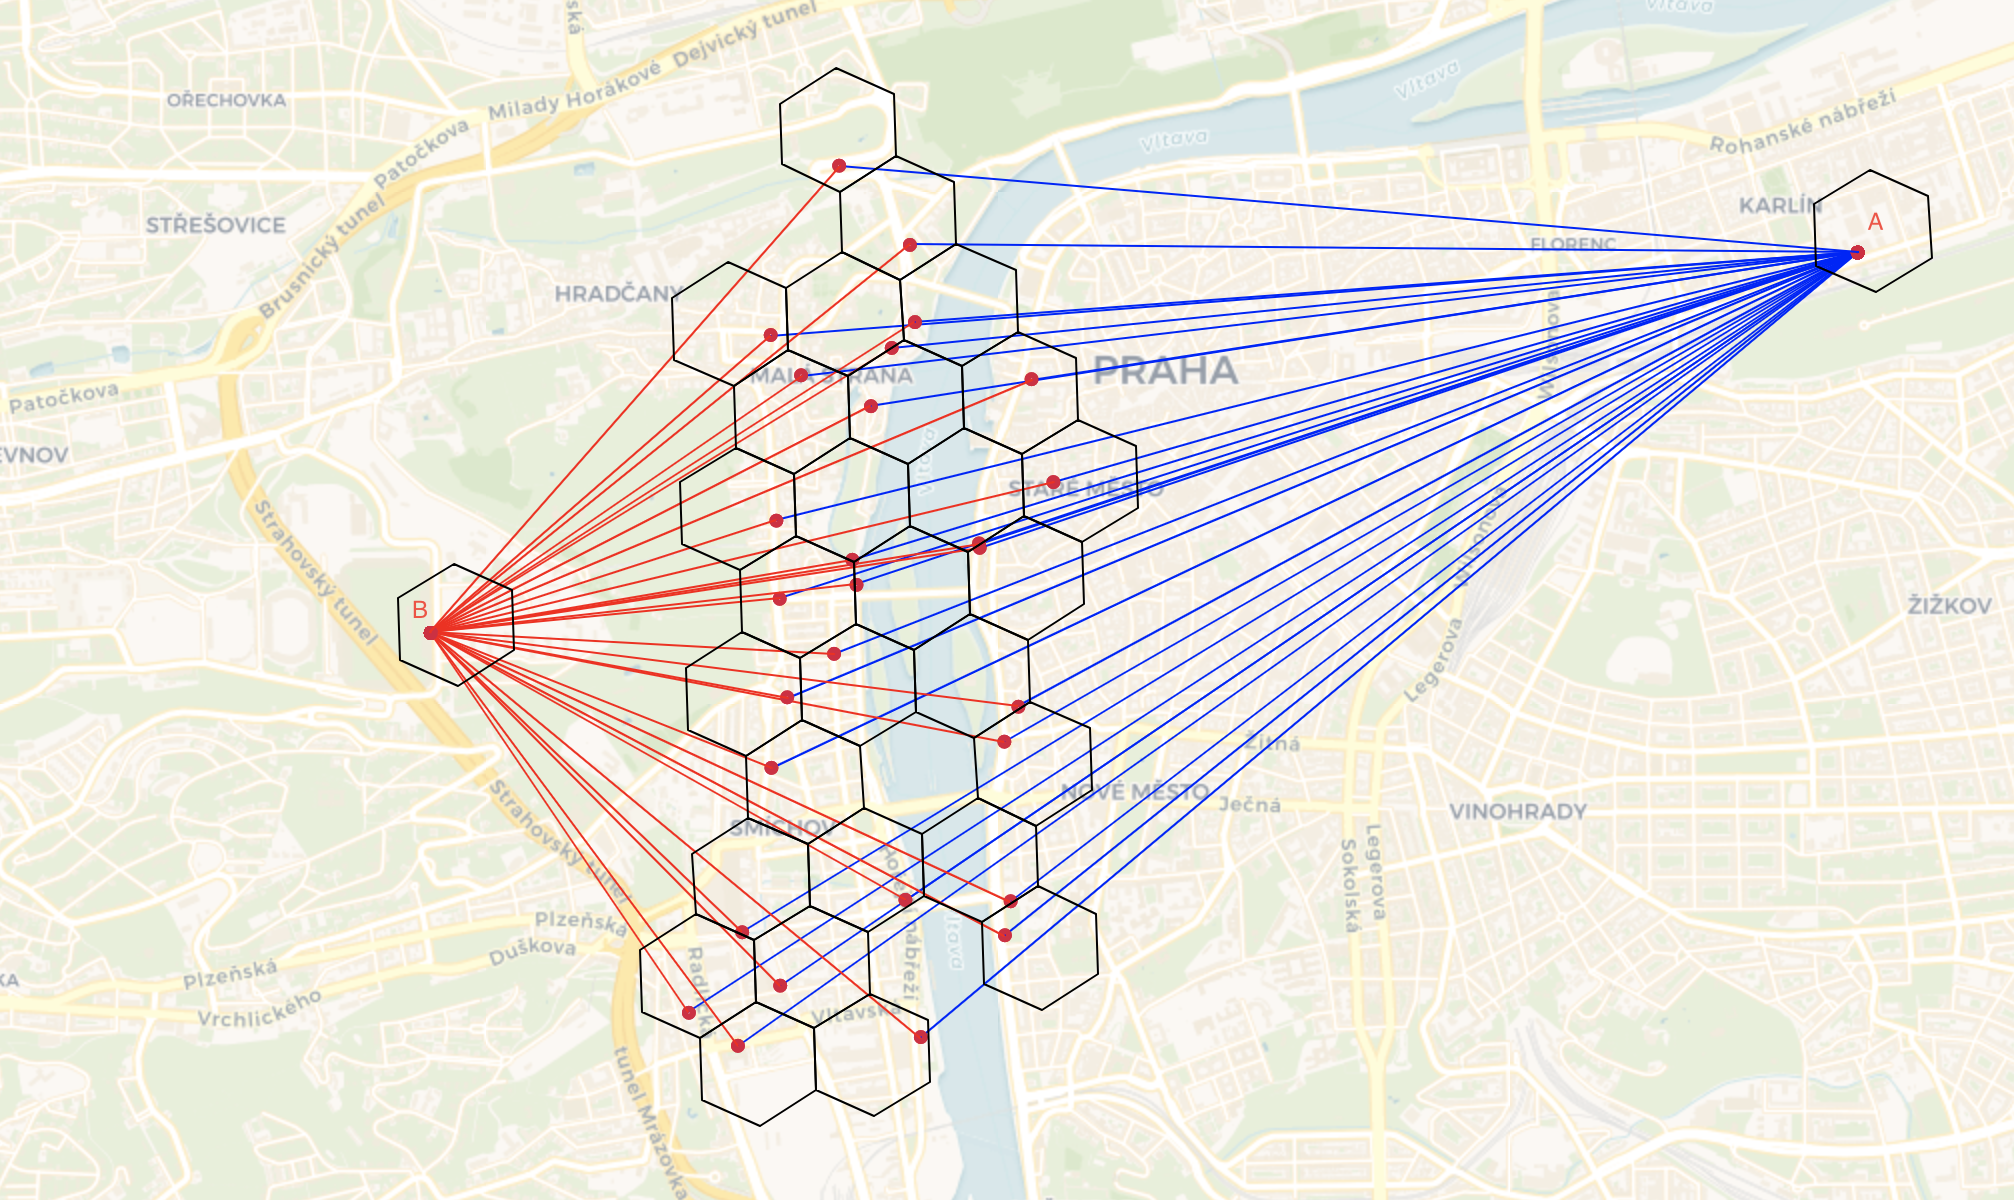
\includegraphics[width=1\textwidth]{graphs/multimodal-last-mile.png}
	
		\caption[Multimodální graf pro plán cesty z bodu A do bodu B, metodou poslední míle. ]{Multimodální graf pro plán cesty z bodu A do bodu B, metodou poslední míle. Černé hexagony obsahují přestupní stanice (Označeny jako červené body). Modré hrany označují zjednodučenou cestu pomocí hromadné dopravy, červené hrany označují cesty pomocí sdíleného prostředku. K vizualizaci grafu je využita knihovna Folium. \cite{folium}}\label{fig:singlemodal-graph}
		% \label{fig:service-zone}
	
	\end{figure}
	


	\item [Krok 8] pomocí Dijskrova algoritmu \footnote{Dijskrův algoritmus je obecně definován kapitole \ref{dijskra}, spolu s konkrétní implementací.} nalezneme základy tras nad HexSpace grafem,

	\item [Krok 9] optimalizujeme výběr prostředku tak, že pro každou etapu cesty, která je plánována sdíleným prostředkem
	\begin{itemize}
		\item vybereme hexagon počátečního bodu a v něm nalezneme nebližší prostředek daného typu a poskytovatele k počátečnímu bodu. Díky tomu minimalizujeme vzdálenost chůze.
	\end{itemize}
	\item [Krok 10] Vrátíme nejlepší základy tras (základem trasy nazývám takovou trasu, která ještě neobsahuje detailní informace o cestě),
	\item [Krok 11] K základům tras konkurentně spočítáme detaily všech etap trasy tak, že
	\begin{itemize}
		\item pro etapy, kde způsob dopravy je sdílený dopravní prostředek nebo chůze, využijeme OSRM backendu,
		\item pro etapy, kde způsob dopravy je veřejná doprava, využijeme OTP backendu.
	\end{itemize}
	\item [Krok 12] Vybereme a vrátíme nejrychlejší cestu.
\end{description}

\subsection{Pomocné funkce plánovače} 

Podkapitola níže popisuje pomocné funkce, které jsou využity k plánování tras.

\subsubsection{Výběr bodů ze servisních zón}\label{vyber-zon}

K manipulaci s prostorovými daty je k výběru nejbližšího bodu v sesrvisní zóně využito knihovny shapely \cite{shapely}. V tomto případě máme nějaký konkrétní bod (buď  cílový bod u singlemodálních cest, nebo cílový krok etapy u multimodálních cest) a nějaký polygon, značící servisní zónu, kam sdílený prostředek můžeme vrátit.

\begin{figure}[H]\centering
	% \includegraphics[width=0.5\textwidth, angle=30]{cvut-logo-bw}
	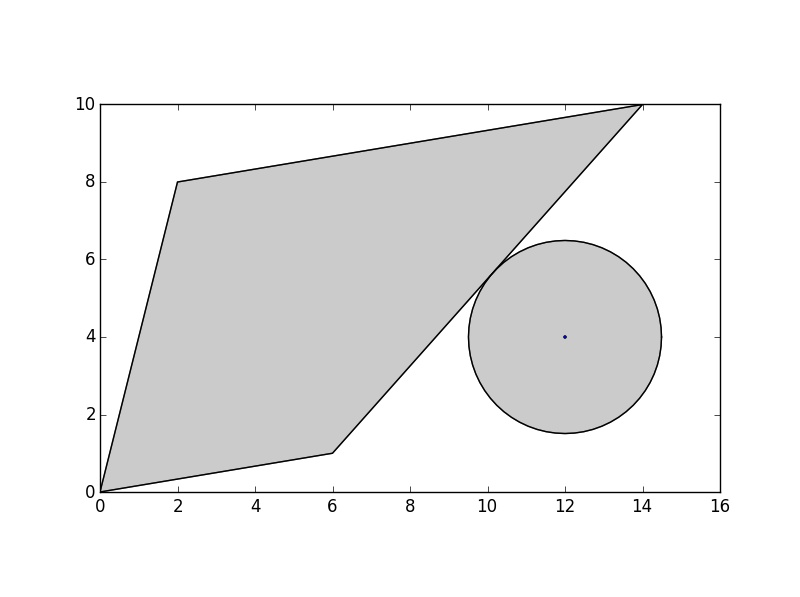
\includegraphics[width=1\textwidth]{graphs/service-zone-selection.jpg}

	\caption[Servisní zóna a bod mimo zónu]{Servisní zóna a bod mimo zónu}\label{fig:service-zone}
	% \label{fig:service-zone}

\end{figure}

Diagram \ref{fig:service-zone} zobrazuje tyto dva objekty. K nalezení nejbližšího bodu v servisní zóně je využito funkce \codeword{nearest_points(geom1, geom2)}, kde \codeword{geom1} a \codeword{geom2} jsou nějaké geometrické objekty.

\subsubsection{Výběr relevantních docků}\label{vyber-docku}

Někteří poskytovatelé sdílené mobility vyžadují, aby jejich vozidla byla vracena ve stojanech. Následující odstavec popisuje, jak relevantní stojany vybrat. Výběr stojanů je poměrně jednoduchý, tedy v okruhu (s předem daným poloměrem) od předem daného bodu zájmu (například cílový bod cesty).

Použitý algoritmus je naivní, tedy, že cyklem procházíme přes všechny stojany, a pro každý stojan spočítáme vzdálenost od bodu zájmu dle Harvesinova vzorce. Pokud je vzdálenost menší, než předem daný poloměr, stojan vybereme pro pozdější výpočty.

Pomocí Harvesinova vzorce\cite{harvesine} je možné spočítat vzdálenost dvou bodů jako vzdálenost dvou bodů po kulové ploše. Harvesinova metoda obsahuje nepřesnost, protože bere jako model kouli (skutečný tvar Země se od tvaru koule mírně liší, což ale na kratších vzdálenostech, jako cesty po městě, je zanedbatelný problém). 



\subsubsection{Výběr tranzitních stanic} \label{vyber-tranzitnich-stanic}

Multimodální cesty jsou realizovány pomocí takzvaných tranzitních (přestupních) stanic. Jako tranzitní stanici můžeme považovat takovou stanici, která je v určité vzdálenosti od bodu zájmu (tato vzdálenost je dána konfigurací). 

V současné době jsou přestupní stanice hledány naivně, tedy cyklem procházíme přes všechny stanice a pro každou stanici spočítáme vzdálenost od bodu zájmu pomocí Harvesinova vzorce\cite{harvesine}. \footnote{Harvesinův vzorec je detailněji popsán v kapitole \ref{vyber-docku}.}
	\begin{itemize}
		\item V případě, že předpoklad platí, stanice je vybrána do dalšího kroku.
	\end{itemize}


% 
% 	- singlemodal 
% - multimodal
% 	- simplifying the graph - transit hubs
% 		- selecting the transit hubs
% 			- naively from the list of stations
% 			- i.e selecting stations from every metro line, bus line, tramline
% 				- spatial search
% 				- geospatial system+search (h3)
% 				- further selection of stations
% 			- TNR selects a subset T ⊂ V (normally 10 000 nodes) of so called transit nodes and stores distances between them in a ta- ble. Moreover, each node v ∈ V stores the distances to all relevant transit nodes, called access-nodes 
% 			- Then, with good choice of T , a long-range query can be reduced to three table lookups. In order to decide whether a query is a long-range query, a locality filter is introduced. In case s and t are too close to each other, an arbitrary speed-up technique is applied. The percentage of global queries can be increased by introducing several layers of transit nodes. 
% 			- 
% 		- fetching times from backends
% 		- connecting the legs
% 		- finding the shortest via cost function
% 	- recreating the route from respective legs

\subsubsection{Získání dat}

% - ziskani dat
% - intro k ziskani dat, 
% - letme popsani sbiraci sluzby, 
% - ulozeni do redisu




\section{Nasazení plánovače}

\subsubsection{Postup kontejnerizace aplikace}

% best practices

\subsubsection{Hardening kontejneru}


\chapter{Architektura plánovače}

TODO uvod kapitoly plus popis nasledujich sekci

% \section{Nasazení aplikace}



\subsection{Koncept mikroslužeb}

Architektura mikroslužeb, jež nabrala na popularitě během posledních let či desetiletí, je způsob návrhu, při kterém míříme k vytvoření množiny malých, lehkých a vzájemně nezáviských služeb. Každá ze služeb běží ve svém procesu nezávislých na ostatních. Všechny služby mezi sebou komunikují na daném mechanismu/protokolu.

Opačným přístupem je monilitická architektura. U monolitického přístupu je celá aplikační logika sepsána jako společný kód (codebase). V případě, že programátor chce změnit jakkoli malou část kódu, je vždy třeba zkompilovat, sestavit a nasadit celou aplikaci. Tato vlastnost monolitické architektury může způsobit komplikace při vývoji aplikace, a to obvzlášť v případě, že aplikace je velká.

I proto jsou automatická nasazení (CI/CD) mnohem jednodužší v architektuře mikroslužeb. V takovém připadě není nutno kompilovat, či sestavovat celou aplikaci, ale pouze změny v dané mikroslužbě, kterou měníme. Jedním z důsledků je i to, že můžeme jednodužšeji se orientovat v kódu aplikace a také jednodužšeji nacházíme a opravujeme chyby (bugy).

Díky tomu můžeme dodávat a nasazovat do produkčního prostředí nové verze aplikace nepoměrně rychleji. Proto je také možno nasazovat menší změny a to s rychlejší frekvencí. 

Dalším problémem monolitické aplikace může být škálování. A to proto, že celá aplikace musí být škálovatelná. U přístupu mikroslužeb, kde každá komponenta, či služba je izolovaná a samostatně škálovatelná, můžeme v případě potřeby naškálovat jen ty části, u kterých je to aktuálně z důvodu vysokého zatížení nutné.

Mezi výhody také patří to, že můžeme jednotlivé instance mikroslužeb rozdělit a distribuovat na několik fyzických strojů, či dokonce datacenter. Pro to, aby služby, co běží na různých serverech, spolu komunikovali, je nutné, aby byl implementovaný Service Discovery protokol. 

V kontrastu k tomu musí být monolitická architektura nasazena na jednom stroji ve stejném prostředí, připadně rozdělena pomocí HA funkcionalit.

% Zde se také dostáváme k problému škálovaní. Monilitická architektura z principu je škálovatelná vertikálně, tedy přidáním hardwarových zdrojů, jako CPU, či paměti RAM. U přístupu mikroslužeb je možno přidání více instancí.

\begin{figure}[H]\centering
	% \includegraphics[width=0.5\textwidth, angle=30]{cvut-logo-bw}
	\includesvg[width=0.5\textwidth]{graphs/microservice-vs-monolith.drawio.svg}

	\caption[Monolitická architektura vs. architektura mikroslužeb]{Monolitická architektura vs. architektura mikroslužeb}\label{fig:float}
\end{figure}


Obrázek výše ukazuje hlavní rozdíly mezi monolitickou a mikroslužbovou architekturou. I přes zjevné výhody architektury založené na mikroslužbách, je nutné podotknout i její nevýhody. Jedním z nich je interní komunikace mezi službami. Ty mohou být implementovány buď jako REST, GraphQl API, či jako RPC volání. Díky tomu by měla být latence mezi službami brána v zřetel. Další věc je, že taková to komunikace vyžaduje stabilní a bezpečnou síť.

Také s tím, jak aplikace založená na mikroslužbách začíná narůstat, začne se objevovat potřeba pro kvalitní monitoring a tracing. Dalším krokem je implementace service mesh komunikace.



\section{Distribuované výpočetní systémy}



\subsection{Virtualizace}

Virtualizace je koncept zavedený již dekády. Koncept odkazuje na vytvoření objektu/zdroje, jako je např. operační systém, hardware, úložiště, či síť, který je na vrstvě abstrahované or reálné vrstvy.

Tyto emulované a virtualizované systémy mohou být nastavovány, udržovány a replikovány mnohem jednodužšeji a na požádání. Další věcí je, že virtualizací jsou zdroje přiřazovány uživatelům, či aplikacím dle jejich reálných potřeb a díky tomu mohou být zdroje mnohem lépe využity. Toto velice pomáhá jak ke snížení nákladů, tak také k šetření životního prostředí. 

Poskytovatelé cloudových služeb, jako Amazon AWS, či Microsoft Azure využívají virtualizace v jiejich datacentrech a následně zdroje nabízejí jako službu (Infrastructure as a service, IaaS). 


Virtualizaci můžeme najít jak na serverové části, tak na té klientské. V této práci budou zmíněny jen ty na serverové části.

Dvě hlavní virtualizační techniky jsou virtualizace založená na hypervisoru a na kontejnerech, které popíšou kapitoly níže.

\subsection{Hypervizor virtualizace}

Virtualizace založená na hypervizorech umožnuje spouštění plných virtuálních strojů (VMs) na hypervisoru. Takové virtuální stroje se skládají z plného operačního systému, obsahujícího kernel (jádro), aplikaci a všechny závislosti. \cite{virt-comparison}

% Hypervisor jako takový je software běžící na hardwaru (např. VMWare ESXi), či jako další vrstva nad operačním systémem (Libvirt/KVM na Linuxu). 

Hypervisory se dále dělí do dvou základních částí, Hypervisor typu 1 a typu 2.

Hypervisor typu 1 (také jako Baremetal Hypervisor) běží přímo na hardwaru daného počítače. Mezi ně patří například Xen, nebo  VMWare ESXi. 

Hypervisory typu 2 (také jako hostovaný hypervisor) běží jako další vrstva nad operačním systémem. Mezi hostované hypervisory patří VirtualBox, QEMU, či VMWare Workstation. Minimálně u platformy x86 roveň oddělení virtuálního stroje od hypervisoru je poměrně robustní, protože CPU instrukce poskytují hardwarovou izolaci a útokový vektor ze strany hypervisoru není tak obrovský. I tak výzkumníci ukázali určité útoky.  



\subsection{Kontejnerová virtualizace}

% + kontejner historie, i.e chroot a solaris zones

Virtualizace založená na kontejnerech (také nazývaná jako virtualizace na úrovni operačního systému, případně kontejnerizace) je odlehčená alternativa k hypervisorům. Tento způsob kontejnerizace využívá funkcí kernelu ze serveru, na kterém virtualizace běží a to tím, že vytváří instance oddělených user-spaců (ve kterých běží skupiny procesů), nazývaných kontejnery. 

Kontejner výpadá z pohledu uvnitř běžícího procesu jako plnohodnotný operační systém. Reálně to ale je oddělený jmenný prostor uvnitř hostujícího operačního systému, se kterým sdílí zdroje (sdílí společný kernel, tedy žádný hypervisor není potřeba). A tedy kontejnery nemají svůj virtualizované hardware (jako např. hypervizor virtualizace). 

Díky tomu, že kontejnery neemulují žádný hardware, nepotřebují čas pro nastartování operačního systému. Proto nabízí velmi rychlé startovací časy (v milisekundách). Kontejner do sebe zabaluje všechny závislosti, které může potřebovat -- jako například knihovny, binární soubory, či jiné konfigurace potřebné k nastavení operačního systému nebo aplikace. Tímto způsobená menší velikost přínáší několik výhod, jako vyšší výkonnost, zvýšenou bezpečnost či dobrou škálovatelnost v porovnání s plnou virtualizací.

Virtualizace založená na kontejnerech může být implementována na jakémkolik operačním systému, každopádně populární techniky, jako třeba Docker jsou založeny na funkcích v Linux kernelu. 


\subsubsection{Mechanismy kontejnerizace}

Kontejnery jsou většinou vytvořeny pomocí následujících funkcí v jádře OS: kernel namespace (jmenný prostor v jádru) a cgroups (Control groups). Tyto funkce se zaměřují na vytváření skupin procesů, které jsou od sebe odděleny (kernel namespaces) a vynucují jim limity na zdroje (control groups).

% V Linuxu je přiřazování zdrojů založeno na cgroups funkcionalitě (control groups).  

Control Groups (or cgroups) jsou využívány na vynucení limitů na hardware zdroje, jako např. počet procesorů, procesorové využití, přiřazení paměti, atp. Taková omezení mohou být přiřazeny buď jednomu procesu, či množině procesů. Cgroups mohou být využity k zajíštění, aby jeden kontejner nezahltil systém využítím všech jeho zdrojů. 

Pravidla jsou organizována ve stromové struktuře, jsou děděny a volitelně vrstvena (nestable).

Cgroups mohou být vnímány jako vylepšení nad ulimity/rlimity. Nastavují se pomocí speciálního virtuálního souboru připojeném v cestě \codeword{/sys/fs/cgroup} a mohou být kdykoliv měněny.

Mezi hlavní skupiny cgroup patří CPU, memory, BLKIO, devices, network nebo freezer. V případě, že jsou špatně nastaveny, tak taková chyba může být využita k útěku z kontejneru ven. 


Právě Docker virtualizaci se se bude věnovat další podkapitola.

\subsection{Docker}

V minulé části jsme popsali kontejnerovou virtualizaci a zde popíšeme reálnou implementaci. Docker přidává abstraktní vrstvu nad koncepty zmíněnými výše. Docker je platforma na vývoj, distribuci a nasazování aplikací. 

Docker se zkládá z těchto funkcí:


\begin{itemize}  
\item Docker Engine (jádro Docker ekosystému)
\item Docker Compose (definice celé infrastrukury pomocí jednoho souboru, nenabízí detailní konfiguraci a proto nebude využit)
\item Docker Swarm (orchestrace kontejnerů na HA klusterech, nebude využito)
\item Docker Registry (úložiště Docker obrazů)
\item Universal Control Plane (management kontejnerů a klusterů v byznys prostředí, nebude využito)
\item Docker Secrets (management hesel ve Swarmu)
\item Docker Content Trust (ukládání a validace značek (tagů) u Docker obrazů)

\end{itemize}


\subsubsection{Docker Engine}

Docker Engine je jádro Docker ekosystému, založený na client-server architektuře, která má 3 hlavní komponenty -- Docker démon, REST API poskytované Docker démonem a CLI klient (příkaz docker).

\paragraph{Docker Daemon}

Docker démon běží na stroji (jako root \footnote{Root je privilegovaný uživatel na Unix-like operačních systémech}) a je zodpovědný za poslouchání na REST API, odkud zpracovává požadavky od Docker klientů. Spravuje také Docker objekty pro kontejnery, obrazy instancí, sítě, diskové objekty.


Existuje také projekt Podman, který nabízí možnost spouštení kontejnerů bez běžícího démona. 

\paragraph{Docker Client}

Docker klient je využíván pro komunikaci s API na démonu. Toto je primární způsob komunikace s démonem.


V této práci je docker využit pro kontejnerizaci plánovací aplikace a poté je nasazen do Kubernetes.

% impl via cgroups, unionfs

% zminit kontejnerizaci bez demona (name?)

% kontejner image + vrstvy

\subsubsection{Architektura Dockeru a komponenty}


\subsubsection{Docker image a Docker kontejner}


Docker obraz\footnote{Docker obraz -- Docker image} je soubor vytvořený z jeho definice či šablony, zvaného Dockerfile.  

\subsection{Frameworky pro orchestraci kontejnerů}


V současné době mezi nejpopulárnější frameworky pro orchestraci kontejnerů patří Docker Swarm, Kubernetes a Apache Mesos. Mezi jejich nejčastěji zmiňované výhody patří vysoká dostupnost při nasazování při použití homogeních prostředí v datacentrech. Z důvodu nejvyšší podpory Kubernetes u cloudových poskytovatelů a také v současnosti největší komunitě se budeme v příštích kapitolách věnovat právě jemu a konkurenční technologie vynecháme.

\subsection{Kubernetes}

Kapitola níže uvede komponenty Kubernetes pro potřeby nasazení plánvací aplikace. Každopádně pro kompletní a více detailní informace doporučuji oficiální dokumentaci. 

Jak definuje oficiální stránka, Kubernetes je orchestrační systém pro kontejnery, navržený pro nasazení, škálování, řízení a kompozici aplikačních konternerů napříč klustery serverů (produkční úrovně). Je to robustní systém pro řízení  kontejnerů, který nabízí virtuální abstrakční vrstvu nad poskytovatelem cloudových služeb a je velmi užitečný pro nasazování a udržování škálovatelných a distribuovaných systémů. Další velkou výhodou je, že pomáhá uživatelům konzistentně nasazovat aplikace na různé aplikační poskutovatele.

Kubernetes je třetí generace služby pro řízení kontejnerů od Googlu, představen na Google Developer Forum v červnu 2014. Kubernetes použil mnoho nápadů z předchozí technologie od Googlu, Borgu. Původně byly aplikace uvnitř Googlu spouštěny právě pomocí Borgu, každopádně později vznikl zájem o podobnou technologii i mimo společnost. Toto motivovalo Google k vývoji právě Kubernetesu.  

\subsubsection{Architektura Kubernetes}


Kubernetes uvádí aplikačně orientovanou architekturu \footnote{AOI -- Application-Oriented Infrastructure}\cite{as-k8s-san-kho-lin} s motivací:

\begin{itemize}  
\item  Co nejvíce zabstraktnit HW stroj a operační systém od aplikace a nasazení 
\item  razí pravidlo jedoho procesu na jeden kontejner. Díky tomu pokud řídíme a ovládáme proces, řídíme i aplikaci. Proto posouvá Kubernetes API z infrastrukturně orientovaného na aplikačne orientovaný a zlepšuje vhled (observability) na aplikace a jejich nasazení
\end{itemize}



% service discovery
% master vs worker node

%  PSP, Network policy
% Calico

% Kubebench

% service mesh


% zabezpeceni kubernetes

\subsubsection{Vlastní nasazení Kubernetes vs Kubernetes as a Service}

Kubernetes je poměrně složitý systém na nasazení a také na následnou údržbu. Nastavení Kubernetes pro běh aplikace v produčním prostředí může být velice zdlouhavé a časově náročné. V případě bezpečnostních chyb v linuxovém jádře je třeba aktualizovat uzly, na kterých běží master i worker služby. Při běhu kubernetes on-premise (tj. na vlastním železe) je třeba takové změny vykonávat ručně.

Poskytovatelé cloudových služeb nabízí kubernetes distribuce u kterých úkoly jako aktualizace Kubernetes, aktualizace operačního systému či například monitoring jsou již automatizované. Takové řešení se nazývá Managed Kubernetes, či Kubernetes as a Service (Kubernetes jako služba). 

Kvůli důvodům zmíněným výše bylo rozhodnuto, že bude využito možností managovaného přístupu ke Kubernetes. Popisu nabídky v roce 2020 a následného výběru nejvhodnější distribuce bude věnována následující kapitola.


\subsubsection{Výběr managované služby}


Kapitola níže popíše nejvíce populární aktuálně dostupné managované distrubuce Kubernetes. Poté bude nastíněn výběr Kubernetes distribuce. V současné době všichni největší poskytovatelé cloudových služeb nabízí managovaný Kubernetes. Některé jsou více integrované do jejich Cloud platformy, některé méně. 

\paragraph{DOKS}

DOKS (Digital Ocean Kubernetes Service)\cite{doks} je distribuce od cloudového poskytovatele Digital Ocean. Mezi hlavní výhody DOKS je rychlost vytvoření clusteru, která je nejkratší ze všech poskytovatelů. Další nespornou výhodou, je, že Kubernetes je poměrně čistý (Vanila Kubernetes) a pro začátečníka takové prostředí může být ideální, protože rozdílů od oficiální dokumentace není mnoho. 

Mezi nevýhody patří poměrně malá nastavitelnost různých parametrů, jako síť, typ load balanceru, atp. 


\paragraph{GKE}

GKE (Google Kubernetes Engine)\cite{gke} je služba nabízená na GCP (Google Cloud Platform). 

		% vysoka integrace ktery vypada nativne (google)


\begin{figure}[H]\centering
	\includesvg[inkscapelatex=false,width=1\textwidth]{graphs/gke-cluster-architecture.svg}

	\caption[Architektura GKE clusteru]{Architektura GKE clusteru}\label{fig:float}
\end{figure}
		
		

\paragraph{EKS}

EKS (Elastic Kubernetes Service)\cite{eks} je služba od AWS (Amazon Web Services). EKS nabízí velké propojení s AWS službami, což s sebou nese výhody, i nevýhody. Výhodou je, že užití EKS je poté téměř bez operačních úkonů a běží bez větších zákroků. Nevýhodou je tzv. vendor-lockin, tj. vysoká komplexita při přechodu z jedné cloudové platformy na druhou.

% integrace s iam

% AWS operators

Nakonec jsem vybral právě EKS díky největším znalostem právě s AWS platformou. Návrh a nastavení clusteru bude popsán v praktické části práce. 

% odkaz na praktickou cast popisujici EKS a AWS komponenty







\subsection{Distribuovaná architektura}


\subsubsection{Softwarově definovaná infrastruktura}

S příchodem cloudu a virtualizace jako takové přišel i nespočet nových nástrojů a platforem, díky kterým začne vznikat portfolio systémů, o které se většinou musíme starat. V důsledku komplexnosti portfolia pomocných programů tedy i krok k více softwarově definované infrastruktuře. Softwarově definovaná architektura (většinou nazývaná jako Infrastructure as Code, zkráceně IaC) je pokus o využití maximálního potenciálu aktuální IT infrastruktury. Kief Morris \cite{kief-morris-iac} popisuje IaC následovně


\begin{quotation}
Infrastruktura jako kód je přístup k administraci IT infrastruktury v době cloudu, s využitím mikroslužeb, automatického nasazování a založeném na praktikách ze softwarového inženýrství.  
\end{quotation}

Pro replikovatelnost řešení této práce budeme používat právě IaC pro popis nasazované infrastruktury.

\paragraph{Výhody IaC}

Využití Softwarově definované architektury má několik hlávních výhod, které jsou popsané níže.


\begin{itemize}  

	\item \textbf{Jednoduše a rychle reprodukovatelné systémy}

	S použitím IaC mohou administrátoři rychle nasadit a nastavit celou infrastrukturu spuštěním jednoho jednoduchého příkazu, či skriptu.

	IaC skripty popisují všechny nutné kroky pro vytvoření požadovaného systému, jako například velikost instance, nainstalovaný software dané verze, nastavení firewallu, atp.

	\item \textbf{Jednorázové systémy} 

	IaC přeměnila starý, statický přístup k systémům na dynamický, kde již neměníme staré instance daného zdroje, ale pro jednoduchost vytvoříme nový. Po ujištění, že nový zdroj pracuje korektně, nahradí starou instanci. Díky tomu je možné programy přesouvat z jednoho serveru na druhý bez velkých potíží. To pomáhá také s aktualizacemi potřebných knihoven nebo operačního systému. Změna způsobu myšlení je proto nutná v případech, kdy potřebujeme dynamicky škálovat systémy a nemůžeme se spolehnout na hardware, na kterém aplikace běží. Obecně jsou tyto dva způsoby administrování architektury nazývány jako cattle (dobytek, tj. nový způsob, kde neřešíme konkrétní instance) versus pets (mazlíčci, tj. starý způsob, kde se o každou instanci staráme jednotilivě). \cite{cattle-pets}

	\item \textbf{Konzistence konfigurace} 

	Lidská práce způsobuje a vždy způsobovala problémy při konzistenci konfigurace. A to i v případech, kdy jsou následovány procesy a postupy. Manuální úpravy vytvoří menší či větší odchylky od původního zdrojového kódu, což zvyšuje pravděpodobnost složitosti a časové náročnosti při opravě softwarové chyby. 

	IaC plně standardizuje konfiguraci infrastruktury a díky tomu nenechává moc prostoru lidské chybě.

	\item \textbf{Sebe se dokumentující systémy} 

	Obvzáště v menších a dynamicky vyvíjených projektech se bojujeme s problémem, že dokumentace není užitečná, nebo nepřesně popisuje daný problém. S tím, jak dokumentaci či program upravujeme, tím je pravděpodobnější nekonzistentnost mezi  dokumentací a kódem programu/infrastruktury. Další problémem je, že různí lidé různě zapisují dokumentaci a jejich vysvětlení problému nemusí být hned čtenáři zřejmé. I díky tomu většina dokumentací přesně nereprezentuje to, co daný problém znamená. IaC toto řeší tím, že definici a dokumentaci generuje přímo z kódu a právě kvůli tomu máme informace vždy aktuální. K tomu je třeba dopsat jen malé části dokumentace k dovysvětlení hůře pochopitelných částí.  

	\item \textbf{Verzování všeho} 

	S tím, jak máme definici infrastruktury v kódu, se nám otvírá možnost použít verzovací systém pro sledování změn, a případně vrácení se ke starší verze infrastruktury, v případě, že se objevily nějaké problémy.

	Verzovací systémy \footnote{VCS -- Version Control System} nám nabízí zobrazení změn, obsahující všechny implementované změny, důvod, a osobu, která změny vytvořila. Taková funkce přidává užitečnost v případě oprav kódu, protože se jednouduše můžeme obrátit na člověka, který danou část změnil. 
\end{itemize}

\paragraph{Terraform}

V našem případě využijeme k popisu infrastruktury program Terraform. Terraform je nástroj na automatizaci infrastruktury od společnosti HashiCorp a je napsán v jazyce Go. Hlavní výhodou Terraformu je, že je multiplatformní, tj. podporuje mnoho různých cílů \footnote{v Terraform terminologii zvané backendy}, mezi němi jsou  cloudoví poskytovatelé, jako AWS, GCP, Azure, ale i bare metal  možnosti nasazení, jako KVM (libvirt) \cite{tf-libvirt}.


Terraform popisuje infrastrukturu pomocí konfiguračních souborů, jež jsou psány v jazyce HCL. Hashicorp Configuration Languag (HCL) je doménově specifický jazyk vyvinutý uvnitř firmy HashiCorp.

\subsubsection{Návrh architektury}

% Architektura systemu a designova rozhodnuti

\begin{figure}[H]\centering
	\includesvg[inkscapelatex=false,width=1\textwidth]{graphs/aws-diagram.drawio.svg}

	\caption[Návrh architektury v AWS cloudu]{Návrh architektury v AWS cloudu}\label{fig:float}
\end{figure}


\subsubsection{Návrh kubernetes clusteru}

\begin{figure}[H]\centering
	\includesvg[inkscapelatex=false,width=1\textwidth]{graphs/kubernetes.drawio.svg}

	\caption[Rozvržení podů a služeb v Kubernetes clusteru]{Rozvržení podů a služeb v Kubernetes clusteru}\label{fig:float}
\end{figure}


% Nasazeni kubernetes


% Pridani secretu do k8s`

% skalovatelnost

%  skalovani podu
% manualni
% autoscaling

\subsection{Automatizace infrastruktury}

Pro zvýšení důvěry ve správnost a kvalitu softwaru, Fowler et al. \cite{microservices-article} doporučuje co nejvíce automatizovat opakované úkoly, jako například spouštění testů, vytváření kontejnerů, či nasazování. Dle jejich názoru by měl CD (continoous deployment) tvořit nasazení doslovně nudným. Také Newman \cite{microservices-book} nazývá virtualizaci jako klíčovým faktorem k automatizaci infrastruktury, a to proto, že napomáhají k aotumatickému vytvoření a škálování virtuálních strojů pro vývojové či produkční prostředí.



\subsection{Vytvoření soukromého Docker registry}

% ECR

% Gitlab Registry


\subsection{API brána}

Když stavíme aplikaci jako množinu mikroslužeb, je nutné se rozhodnout, jak klienti aplikace budou komunikovat s jednotlivými mikroslužbami. S monolitickou aplikací máme pouze jeden (většinou replikovaný a load-balancovaný) endpoint. V architektuře mikroslužeb každá služba množinu svých endpointů. V kapitole níže představíme, jak tento přístup ovlivňuje komunikaci mezi aplikací a klientem, dále představíme návrhový vzor zvaný API brána.  

 \paragraph{Přímá komunikace mezi mikroslužbou a klientem}

 \paragraph{Využití brány}



\subsubsection{Výběr API brány}
\subsubsection{Vytvoření loadbalanceru}
\subsubsection{Přiřazení DNS záznamu}


\begin{figure}[H]\centering
	\includesvg[inkscapelatex=false,width=1\textwidth]{graphs/api-gateway.drawio.svg}

	\caption[Diagram komunikace klienta se službou]{Diagram komunikace klienta se službou}\label{fig:float}
\end{figure}



% traefik 
\subsection{Nastavení sítě}

Diagram níže popisuje rozvržení sítě po plánovací aplikaci v cloudové platformě AWS. Základní oddělovací částí v AWS je VPC (Virtual Private Cloud)\cite{aws-vpc}, umožňující vytvoření logicky izolované části AWS cloudu do které se nasazují AWS zdroje dle nastavení virtuální sítě.

\begin{figure}[H]\centering
	\includesvg[inkscapelatex=false,width=1\textwidth]{graphs/vpc.drawio.svg}

	\caption[Rozvržení subnetů využitých pro aplikaci v jednom AWS regionu]{Rozvržení subnetů využitých pro aplikaci v jednom AWS regionu}\label{fig:float}
\end{figure}

Pro plánovací aplikaci využíváme jednoho AWS regionu, který se obvykle skládá ze tří dostupnostních zón (AZ, Availability zones)\cite{aws-azs}. Každá dostupnostní zóna je jedno či více datacenter v jednom regionu, datacentra jsou navíc stavěna tak, aby každá z nich byla vystavěna jiným živelným rizikám. Tedy pro příklad, pokud je jedna dostupnostní zóna náchylná povodním, druhá AZ bude stavěna na kopci. Podobně to funguje s energetickým mixem či síťovým připojením. 


Jak je zřejmé z diagramu, v našem případě vytváříme v každé AZ jeden soukromý a jeden veřejný subnet. Co subnety obsahují bude diskutováno v následujících kapitolách.

\subsection{Zabezpečení Kubernetes clusteru}

% Principle of Least Privilege

\subsubsection{Princip nejméně privilegovaného}

Již v roce 1975 Saltzer a Schroeder poznamenali, že každý program a každý uživatel nějakého systému by měli operovat s využitím nejmenší množiny privilegií, která jsou nutná k vykonání nějakého úkonu. \cite{least-priv1} Striktní následování principu nejméně privilegovaného předcházíme bezpečnostním problémům, jako privilege creep (privilegovaný slídil, \cite{least-priv3}). Bohužel porušení tohoto principu jsou poměrně častá \cite{least-priv2}, kde mezi hlavní důvody patří neznalost zabezpečitelnosti, otevřená privilegia pro budoucí použití, či nezabezpečené počáteční nastavení.

V AWS je využito principu nejméně privilegovaného při vytváření IAM uživatelů a rolí \cite{aws-iam}. Tedy je nutné určit, jaké minimální oprávnění uživatel vyžaduje a vytvořit taková pravidla, aby byl schopen vykonat pouze takové úkony. Stejným principem budeme přiřazovat přístupy ke zdrojím v Kubernetes clusteru, kde využijeme RBAC \cite{k8s-rbac}.

Standardním procesem je přiřazení minimální množiny oprávnění a následně přidávat další potřebná. Tento přístup je bezpečnější, než přiřazení počátečních pravidel, která jsou moc volná a následně  se je snažit utahovat. 


\paragraph{Přiřazení Kubernetes RBAC rolí k IAM účtům}

Ke Kubernetes clusteru je třeba administrativní přístup, ať už při hledání různých chyb, či pro monitoring systému. Pro zjednodušení administrace účtů je třeba  mít single source of truth (SSOT), kde jsou účty uloženy. Jako úložiště je přirozeně v AWS ekosystému vybráno IAM -- a účty v Kubernetes jsou na ně pomocí RBAC namapovány. Mapování uživatelů je detailně popsáno v \cite{iam-rbac-mapping}.

Role jsou namapovány 

\paragraph{Přiřazení IAM rolí k podům v Kubernetes}

K přiřazení IAM rolí k podům v Kubernetes je využito open source nástroje Kube2IAM \cite{kube2iam-github}.  Kube2IAM byl první kandidát na vyřešení problému přiřazení IAM rolí ke Kubernetes zdrojům. Nástroj je nasazen na každý uzel Kubernetes jako DaemonSet. 
DaemonSet běží v privilegovaném bezpečnostním módu, takže může vytvářet \codeword{iptables} pravidla, kterými odchytává požadavky na EC2 Metadata, běžící na adrese \codeword{169.254.169.254}. Kube2IAM pody tedy na každém Kubernetes uzlu odposlouchávají požadavky na IAM API. Místo toho, aby  autentizovali napřímo, assumují ("osvojují si") role, které jsou k podům přiřazeny pomocí anotací. Následovně odpoví s dočasnými přístupovými údaji z assumované role. Žádné změny nejsou nutné a aplikace může běžet tak, jak byla navrhnuta pro čistý Kubernetes.

\begin{figure}[H]\centering
	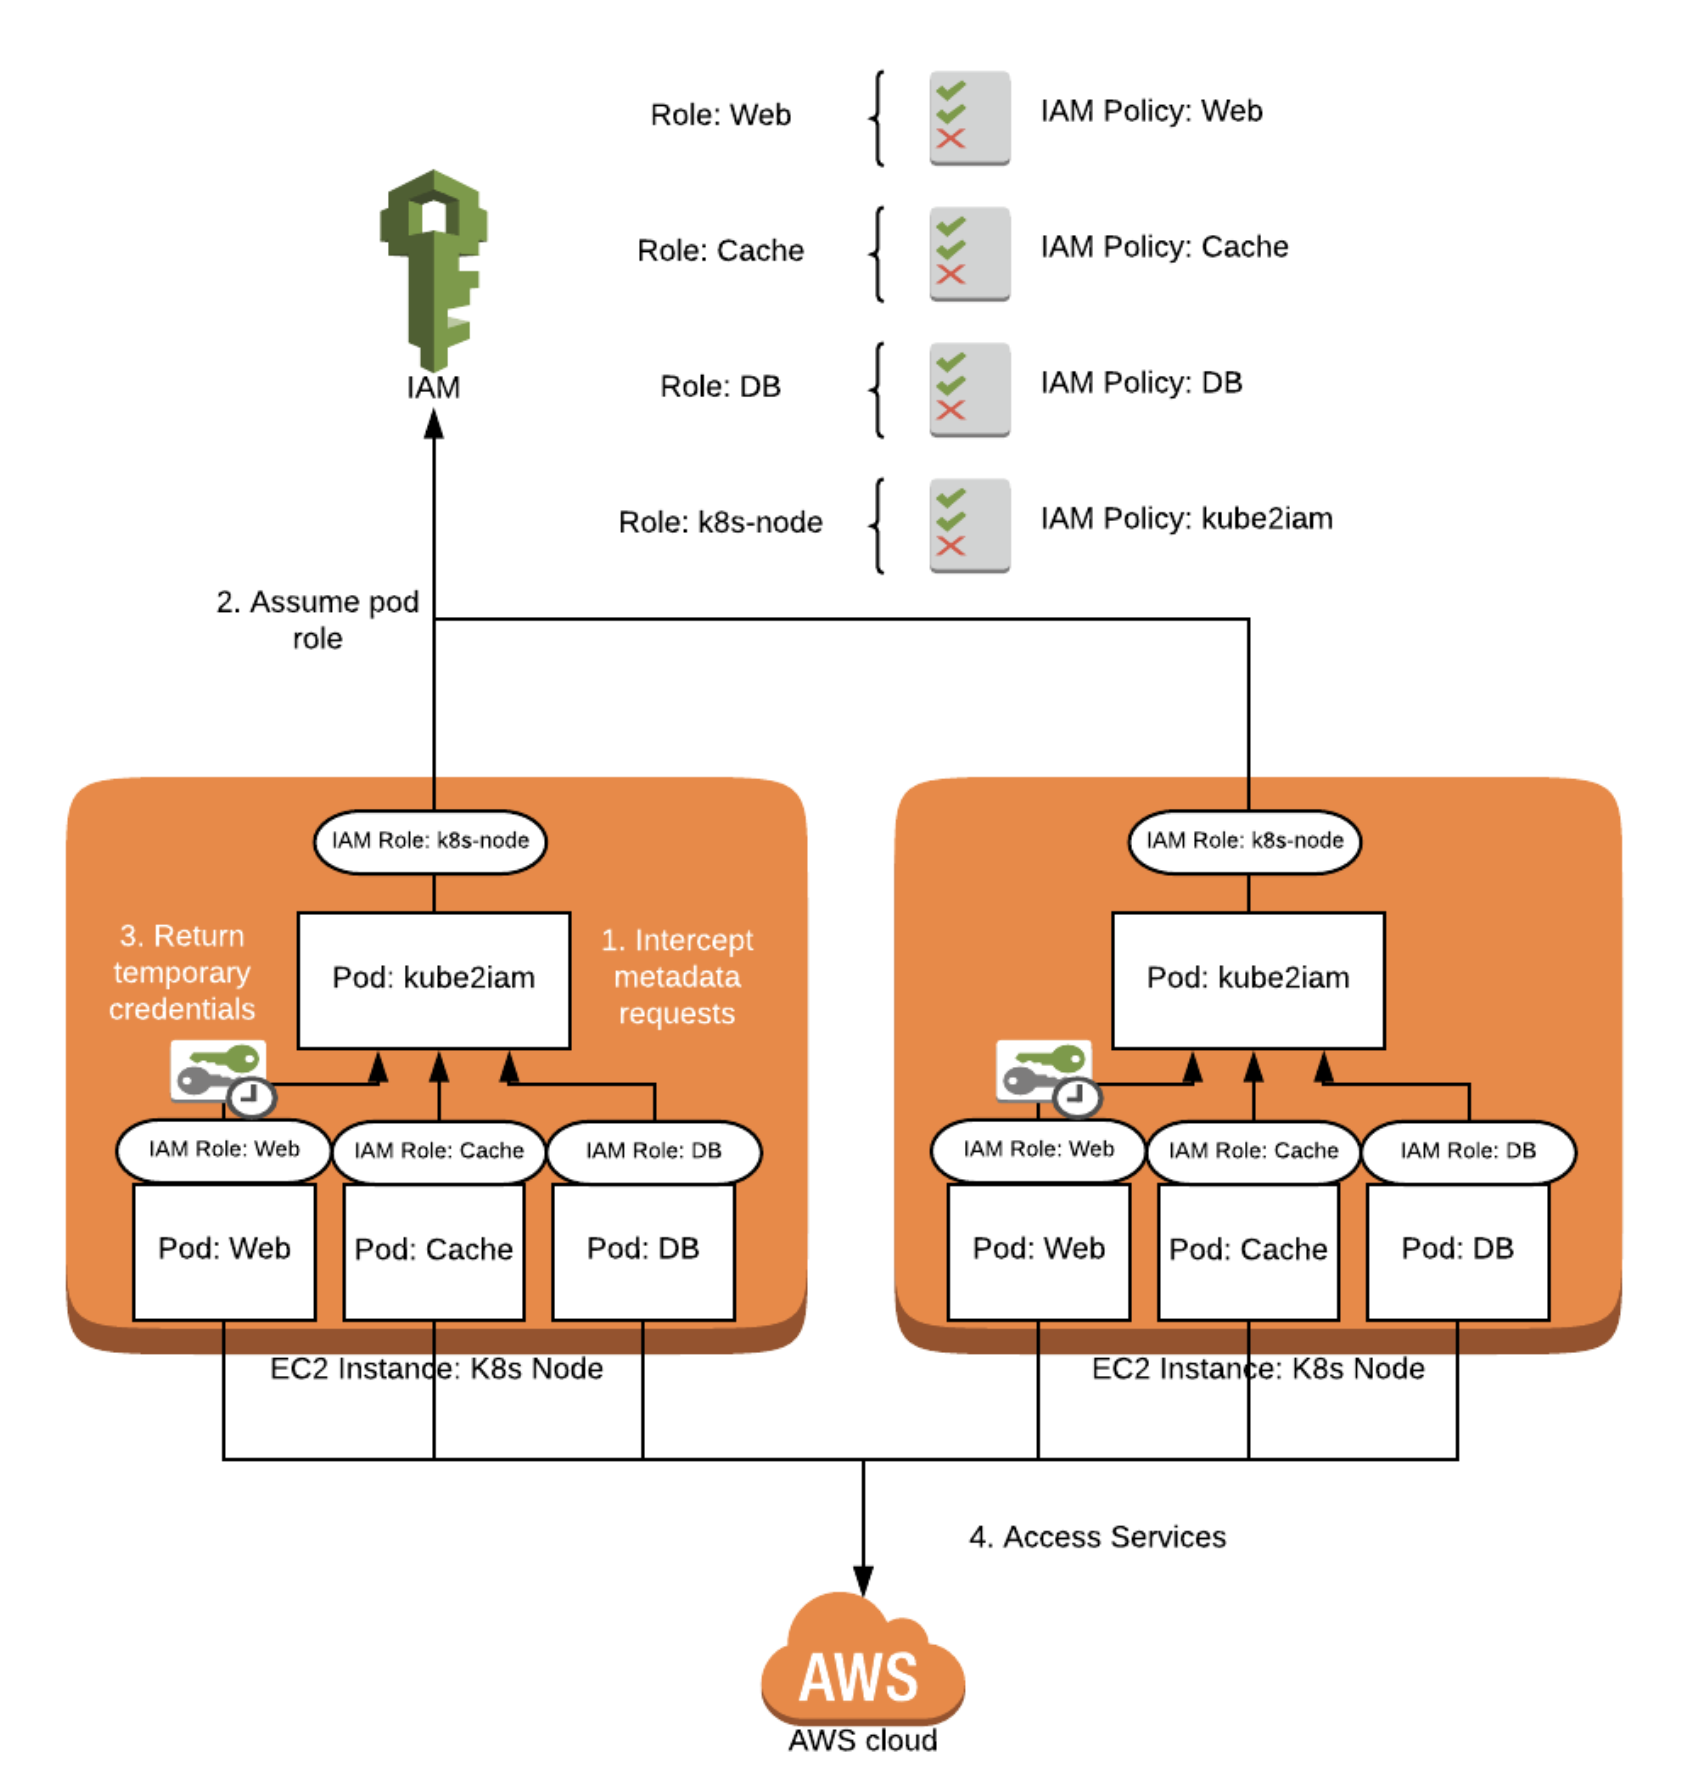
\includegraphics[width=1\textwidth]{graphs/kube2iam.png}

	\caption[Přiřazení IAM práv, komunikace mezi podem a IAM API]{Přiřazení IAM práv, komunikace mezi podem a IAM API}\label{fig:float}
\end{figure}



Existuje několik alternativ ke Kube2IAM. Jedním z nich je Kiam \cite{kiam-github}, který je silně inspirovaný právě Kube2IAM. Kiam jako projekt je ještě více bleeding-edge, a jako projekt je o něco méně aktivní. Kiam řeší škálovací problémy a problémy se zabezpečením, které byly obsaženy v Kube2IAM v době vytvoření Kiam. Řeší to následovně -- rozděluje svoji činnost na serverovou část a agent část. Agent běží jako DaemonSet a zachytává komunikaci s EC2 metadatami, podobně jako u Kube2IAM. Rozdíl je ten, že klient nekomunikuje přímo s IAM, ale tuto práci přenechává na svoji server část. Blogový článek od vývojáře Kiam problematiku popisuje více do detailu. \cite{kiam-post} 


Další alternativou je přiřazení IAM rolí přímo na uzly Kubernetes workerů. Toto má jednu hlavní bezpečnostní nevýhodu -- každý pod, který na daném uzlu beží, je schopen vykonávat úkony, které mu IAM role povoluje. Díku tomu tato možnost byla hned zavrhnuta.  

Poslední časou využívanou variantou je využití federace autentizace pomocí OICD (OpenID Connect). \cite{eks-oidc} Této metody nebylo využito kvůli vendor lock-inu daného řešení.





\section{Continuous Integration \& Continuous Deployment}

Podkapitolky níže popíšou koncepty Continuous integration, Continuous delivery (dohromady také zvané jako CI/CD), dále ukážou současnou nabídku takových služeb. Dále bude jedna ze služeb vybrána a její technologie bude diskutována.

% TODO: teoreticky popis
\subsection{Continuous integration}

Cílem Continuous integrace (CI) \cite{fowler-ci}je propojení práce developera (jako například kompilace aplikace, sestavení kontejneru, spuštění testů) a kódu aplikace. Tato integrace by se měla dít s vyšší frekvencí, např. nekolikrát denně, či po každém commitu do repozitáře s kódem.

Částí CI procesu může být i kontrola kódu (code review) od kolegů developerů.

Výstupem CI procesu je připravená verze aplikace (např. tedy binární soubor nebo kontejner), který se nazývá artefakt (artifact).


Častá integrace a kvalitní testové pokrytí pomáhá s důvěrou v kód na straně jak developerů, tak i na straně serverových administrátorů. 

\subsection{Continuous delivery}

Continuous delivery (CD) je v podstatě automatizace nasazení aplikací a řadí se za Continuous integration. CD tedy popisuje možností nasazení artefaktů z CI do různých aplikačních prostředí, jako je např. produkce.\cite{humble-ci}

Každý tým má různé potřeby při stavění takových CD. Někde je třeba více testovacích (develop) prostředí, jiné týmy vyžadují mnoho staging (prostředí identické produkčnímu ale bez reálné zátěže) prostředí. Při CD vytvoření takového prostředí může být plně automatizováno, případně se může jednat o několik (potvrzujících) kliknutí.

% Gitlab CI
% Jenkins
% Circle CI

\subsection{Návrh CI/CD pro plánovací službu}

Diagram níže ukazuje CI/CD proces pro plánovací službu z této práce.



\begin{figure}[H]\centering
	\includesvg[inkscapelatex=false,width=1\textwidth]{graphs/CICD.drawio.svg}

	\caption[Diagram v CI pipeline]{Diagram v CI pipeline}\label{fig:float}
\end{figure}

Kód aplikace je uložen v git repozitáři na serveru GitHub. Po zapsání změn do repozitáře se spustí Unit Testový krok a pokud proběhne úspěšně, z aplikace se začne vytvářet kontejner. V případě, že změny jsou v master, staging, či develop branchi, tak obraz je pushnut do kontejner repozitáře (ECR). CD proces poté čeká na vstup od uživatele, který svým schválením může aplikaci nasadit do respektivních prostředí.


\section{Nasazení aplikace}

Kapitola níže popisuje praktické nasazení aplikace do distribuovaného prostředí Kubernetes. Ukáže, které Kubernetes zdroje jsou potřebné a jak je možné proces automatizovat s nástrojem Helm. 


\subsection{Helm}

Standardním způsobem definování zdrojů v Kubernetes clusteru je vytvoření konfiguračního souboru pro každý zdroj. V případě, kdy spouštíme aplikaci s různým nastavením (jako produkční a testovací prostředí, atp.), bychom museli jednotlivé konfigurační soubory duplikovat. Tím míříme k redundantnímu kódu, kterému se chceme vyhnout (pokud dodržujeme DRY \footnote{DRY -- Do not repeat yourself} pravidlo).

K nasazení je využito nástroje Helm \cite{helm-docs}.

Helm pomáhá s vytvořením dynamických konfiguračních souborů s použitím proměnných. Helm používá Go Template Engine, kterým generuje Kubernetes zdroje s využitím předem definovaných proměnných. Právě kvůli tomu můžeme vytvořit pouze jeden resource template (šablonu Kubernetes zdroje), ze kterého se vygenerují lehce odlišné zdroje pro každé prostředí. 

Využijeme Helmu verze 3, který všechny změny vypočítává na klientské části (na počítači u vývojáře), což je změna oproti verzi druhé, kde bylo třeba nasazovat Tiller (server část Helmu v2) do Kubernetes.

\subsection{Kubernetes objekty}


Jak bylo zmíněno v teoretické části práce, Kubernetes byl navrhnut jako desired state model a ten je možno definovat několika typy předpisů, mezi které patří například YAML a JSON. My využijeme YAML formátu. Tento předpis bude verzovaný a generovaný pomocí Helmu zmíněného výše. Desired state konfigurace by se dala také nazvat jako spustitelná dokumentace, ze které můžeme kdykoliv obnovit nastavení Kubernetes objektů. 

Aplikace obsahuje tyto Kubernetes objekty:

\paragraph{Deployment}
\paragraph{Service}
\paragraph{Ingress}
\paragraph{IngressRoute}
\paragraph{ServiceMonitor}
% \paragraph{ServiceMonitor}

\section{Škálování aplikace}

% Popis jak skalovat

\subsection{Bezstavová aplikace}

% Popis ze aplikace je bezstavova, tj. neni treba zadna komunikace mezi jednotlivymi replikami

\subsection{Horizontální škálování}
\subsubsection{Horizontální škálování uzlů clusteru}
\subsubsection{Horizontální škálování podů}

\subsection{Vertikální škálování}



\chapter{Možná vylepšení do budoucnosti}
Kapitola níže popisuje možná vylepšení a je rozdělena na vylepšení na aplikaci a na vylepšení na infrastruktuře.

\section{Vylepšení na plánovací aplikaci}

\subsection{Návrh nejkratších cest s ohledem na dopravní zácpy}


% - Možná vylepšení do budoucnosti
%     - vylepseni na routingu
%         - návrh nejkratších cest s ohledem na dopravní zácpy 
%             - pouziti traffic dat
%         - návrh cest dle jiných cenových funkcí (tedy místo nejkratší to “nejpříjemnější” - okolo zelených parků, případně málo vytížených ulic, atp) 
%             - upravy cenove funkce
%         - použití nových algoritmů pro navigaci
%         - zrychlovani
%     - vylepseni na architekture


\section{Vylepšení na architektuře}



\subsection{Service mesh}


\subsection{OIDC}



% \chapter{Realizace}

\begin{conclusion}
	%sem napište závěr Vaší práce
\end{conclusion}

\bibliographystyle{csn690}

\bibliography{mybibliographyfile}

\begin{thebibliography}{9}

\bibitem{zaklady-teorie-grafu}

Základy Teorie Grafů pro (nejen) informatiky, Doc. RNDr. Petr Hliněný, Ph.D., Fakulta Informatiky Masarykova Univerzita, 2010

\bibitem{multimodal-route-planning}

Multi-Modal Route Planning, Thomas Pajor, Institut fur Theoretische Informatik, Universitat Karlsruhe (TH), Germany, 2009

\bibitem{route-planning-in-transportation-networks}
Route Planning in Transportation Networks, HANNAH BAST, DANIEL DELLING, ANDREW V. GOLDBERG, MATTHIAS MÜLLER-HANNEMANN, THOMAS PAJOR, PETER SANDERS, DOROTHEA WAGNER, RENATO F. WERNECK, Microsoft Research, 2014

\bibitem{modelling-of-preferences-in-multimodal-routing-algorithms}

Modelling of preferences in multimodal routing algorithms, Santtu Saijets, Master’s Thesis, Aalto University, 2018

\bibitem{time-dependent-networks-as-models-to-achieve-fast-exact-time-table-queries}

Gerth Stølting Brodal and Riko Jacob. Time-dependent networks as models to achieve fast exact time-table queries. Electronic Notes in Theoretical Computer Science, 92:3–15, 2004.


\bibitem{virt-comparison}

M. J. Scheepers, “Virtualization and containerization of application infrastructure: A comparison,” in 21st Twente Student Conference on IT, vol. 1,
pp. 1–7, 2014.

\bibitem{monitoring-smart-cities}

S. Muralidharan, G. Song, and H. Ko, “Monitoring and managing iot applications in smart cities using kubernetes,” CLOUD COMPUTING 2019,
p. 11, 2019.

\bibitem{k8s-avail-manager}

L. A. Vayghan, M. A. Saied, M. Toeroe, and F. Khendek, “Kubernetes as an availability manager for microservice applications,” 1901.04946, 2019.

\bibitem{microservice-devops}

A. Balalaie, A. Heydarnoori, and P. Jamshidi, “Microservices architecture enables devops: Migration to a cloud-native architecture,” Ieee Software, vol. 33, no. 3, pp. 42–52, 2016.


\bibitem{microservice-docker}

] D. Jaramillo, D. V. Nguyen, and R. Smart, “Leveraging microservices architecture by using docker technology,” in SoutheastCon 2016, pp. 1–5, IEEE,
2016.

\bibitem{docker-reproducible}

C. Boettiger, “An introduction to docker for reproducible research,” ACM
SIGOPS Operating Systems Review, vol. 49, no. 1, pp. 71–79, 2015.

\bibitem{cloud-native-experience}

	A. Balalaie, A. Heydarnoori, and P. Jamshidi, “Migrating to cloud-native
architectures using microservices: an experience report,” in European Conference on Service-Oriented and Cloud Computing, pp. 201–215, Springer,
2015.
\bibitem{ha-k8s}



Elastisys, “Setting up highly available kubernetes clusters.”
https://elastisys.com/wp-content/uploads/2018/
01/kubernetes-ha-setup.pdf. [Online


\bibitem{priv-container}

	Jesse Hertz. Abusing privileged and unprivileged linux containers. Whitepaper,
	NCC Group, 2016.

\bibitem{hardening-container}

	Aaron Grattafiori. Understanding and hardening linux containers. Whitepaper,
NCC Group, 2016.

\bibitem{microservices-article}

Martin Fowler and James Lewis. Microservices. https://martinfowler.com/
articles/microservices.html, 2014. Accessed: 29.08.2017

\bibitem{microservices-book}

Sam Newman. Building microservices: designing fine-grained systems. ” O’Reilly
Media, Inc.”, 2015.

\bibitem{docker-saigon}

Docker Saigon. Docker internals. http://docker-saigon.github.io/post/
Docker-Internals/, 2016. Accessed: 23.07.2017., 

\bibitem{as-k8s-san-kho-lin}


San Kho Lin, Auto-scaling an optimisation algorithm using Docker and Kubernetes on the NeCTAR Research Cloud, UNIVERSITY OF MELBOURNE, 2018


\bibitem{aws-vpc}


\url{https://docs.aws.amazon.com/vpc/latest/userguide/what-is-amazon-vpc.html
}

\bibitem{aws-azs}

\url{https://docs.aws.amazon.com/AWSEC2/latest/UserGuide/using-regions-availability-zones.html#concepts-availability-zones
}

\bibitem{fowler-ci}

Fowler, Martin. Continuous Integration. martinFowler.com. [online], May 1,
2006 [cit. April 2, 2020]. Available from https://martinfowler.com/articles/
continuousIntegration.html.

\bibitem{humble-ci}

Humble, Jez. Continuous Delivery - Priciples. continuousdelivery.com. [online],
2017 [cit. April 2, 2020]. Available from https://continuousdelivery.com/
principles/
\bibitem{helm-docs}

https://helm.sh/docs/


\bibitem{kief-morris-iac}

Infrastructure as Code: Managing Servers in the Cloud
Přední strana obálky
Kief Morris
O'Reilly Media, 2016 - Počet stran: 336

\bibitem{tf-libvirt}

https://github.com/dmacvicar/terraform-provider-libvirt

\bibitem{gtfs-spec}

Google Developers. GTFS Static Overview | Static Transit | Google Developers. [Online; accessed 6-February-2017]. 2020.

\bibitem{otp-api-spec}

http://dev.opentripplanner.org/apidoc/1.0.0/index.html

\bibitem{k8s-up-and-running}

Hightower, Kelsey, Brendan Burns, and Joe Beda. Kubernetes: up and running: dive into the future of infrastructure. 1 ed. USA: O’Reilly Media, Inc, 2017.
ISBN 9781491935675.


\bibitem{oss-benchmark-microservices}

Gan, Yu, Yanqi Zhang, and Dailun Cheng et al. An Open-Source Benchmark
Suite for Microservices and Their Hardware-Software Implications for Cloud \&
Edge Systems. In: International Conference on Architectural Support for Programming Languages and Operating Systems - ASPLOS. 2019. ISBN 9781450362405.


\bibitem{otp-site}


http://docs.opentripplanner.org/en/dev-2.x/


\bibitem{gtfs-prague}


\url{https://opendata.praha.eu/dataset?organization=dpp&res_format=GTFS}


\bibitem{lgpl}

http://www.gnu.org/licenses/lgpl-3.0.en.html


\bibitem{lgpl-stallman}

http://www.gnu.org/licenses/why-not-lgpl.html

\bibitem{osrm-webpage}

http://project-osrm.org/

\bibitem{cattle-pets}

https://www.hava.io/blog/cattle-vs-pets-devops-explained


\bibitem{doks}

https://www.digitalocean.com/docs/kubernetes/


\bibitem{gke}
https://cloud.google.com/kubernetes-engine/docs/concepts/cluster-architecture


\bibitem{eks}
https://docs.aws.amazon.com/eks/latest/userguide/clusters.html


\bibitem{h3}

https://eng.uber.com/h3/


\bibitem{discrete-global-grid}

Geodesic Discrete Global Grid Systems
Kevin Sahr, Denis White, and A. Jon Kimerling
http://webpages.sou.edu/~sahrk/sqspc/pubs/gdggs03.pdf

\bibitem{shapely}

https://shapely.readthedocs.io/en/stable/manual.html


\bibitem{shapely-nearest-points}


\url{https://shapely.readthedocs.io/en/stable/manual.html#shapely.ops.nearest_points}

\bibitem{harvesine}

MĚŘENÍ VZDÁLENOSTÍ A PLOCHY POMOCÍ GPS, DIPLOMOVÁ PRÁCE,  Bc. JAKUB KONECKÝ, 2009


\bibitem{osrm-table-api}

\url{http://project-osrm.org/docs/v5.5.1/api/#table-service}

\bibitem{osrm-route-api}

\url{http://project-osrm.org/docs/v5.5.1/api/#route-service}


\bibitem{spp-def}

Algoritmy pro hledání nejkratších cest
v neorientovaných grafech , BAKALÁŘSKÁ PRÁCE
Richard Benkovský , 2007, MASARYKOVA UNIVERZITA
FAKULTA INFORMATIKY 

\bibitem{least-priv1}

Jerome H. Saltzer and Michael D. Schroeder. The Protection of Information in
Computer Systems. 1975.


\bibitem{least-priv2}

Gary McGraw and John Viega. Software security principles, Part 3: Controlling access - Least privilege and compartmentalization. http://www.ibm.com/
developerworks/library/se-priv/index.html, November 2000.

\bibitem{least-priv3}

Security Threats: A Guide for Small and Medium Businesses. Whitepaper,
GFI, 2009.
\bibitem{iam-rbac-mapping}

https://docs.aws.amazon.com/eks/latest/userguide/add-user-role.html


\bibitem{kiam-post}

https://medium.com/@pingles/kiam-iterating-for-security-and-reliability-5e793ab93ec3 

\bibitem{eks-oidc}

https://docs.aws.amazon.com/eks/latest/userguide/iam-roles-for-service-accounts-technical-overview.html 

\bibitem{kiam-github}

https://github.com/uswitch/kiam


\bibitem{kube2iam-github}


https://github.com/jtblin/kube2iam


\bibitem{aws-iam}

https://docs.aws.amazon.com/IAM/latest/UserGuide/introduction.html


\bibitem{k8s-rbac}
https://kubernetes.io/docs/reference/access-authn-authz/rbac/

\bibitem{first-last-commute}

"Using Bicycles for the First and Last Mile of a Commute" (PDF). Mineta Transportation Institute. September 2009. Retrieved 24 October 2011.

\bibitem{first-last-commute2}

DeMaio, Paul (2009). "Bike-sharing: History, Impacts, Models of Provision, and Future" (PDF). Journal of Public Transportation. 12 (4): 41–56. doi:10.5038/2375-0901.12.4.3. Archived from the original (PDF) on 1 October 2017. Retrieved 24 October 2011.

\bibitem{first-last-commute3}

Shaheen, Susan; Guzman, S., and H. Zhang (2010). "Bikesharing in Europe, the Americas, and Asia: Past, Present, and Future" (PDF). Transportation Research Record: Journal of the Transportation Research Board. doi:10.3141/2143-20. S2CID 40770008. Archived from the original (PDF) on 10 June 2012.


\bibitem{folium}

https://python-visualization.github.io/folium/
\end{thebibliography}


\appendix

\chapter{Seznam použitých zkratek}
% \printglossaries
\begin{description}
	\item[GUI] Graphical user interface
	\item[XML] Extensible markup language
\end{description}
 

\chapter{Obsah přiloženého CD}

%upravte podle skutecnosti

\begin{figure}
	\dirtree{%
		.1 readme.txt\DTcomment{stručný popis obsahu CD}.
		.1 exe\DTcomment{adresář se spustitelnou formou implementace}.
		.1 src.
		.2 impl\DTcomment{zdrojové kódy implementace}.
		.2 thesis\DTcomment{zdrojová forma práce ve formátu \LaTeX{}}.
		.1 text\DTcomment{text práce}.
		.2 thesis.pdf\DTcomment{text práce ve formátu PDF}.
		.2 thesis.ps\DTcomment{text práce ve formátu PS}.
	}
\end{figure}



\end{document}
